% ---------------------------------------------------------------------------
% Follow-Up Is Not Discovery: What a Record of Prior Audit Findings Can and
% Cannot Tell You.  Anonymized manuscript source.
%
% Build: make  (pdflatex + bibtex).  Every number in the prose is a macro
% defined in exhibits/numbers.tex, generated from verified outputs; nothing
% is typed by hand.  See README.md.
% ---------------------------------------------------------------------------
\documentclass[12pt]{article}

\usepackage[T1]{fontenc}
\usepackage[utf8]{inputenc}
\usepackage[american]{babel}
\usepackage[margin=1in]{geometry}
\usepackage{mathptmx}
\usepackage{amsmath}
\usepackage{amssymb}
\usepackage{amsthm}
\usepackage{booktabs}
\usepackage{graphicx}
\usepackage{natbib}
\usepackage{setspace}
\usepackage{url}
% Journal convention: text, references, then figures and tables.
\usepackage[nolists,nomarkers,figuresfirst]{endfloat}
\renewcommand{\efloatseparator}{\mbox{}}

\bibliographystyle{plainnat}
\setcitestyle{authoryear,round}

\setlength{\emergencystretch}{1em}
\graphicspath{{exhibits/}}
\renewcommand{\thesection}{\arabic{section}}

\theoremstyle{definition}
\newtheorem{proposition}{Proposition}[section]

% Generated by scripts/s1_exhibits.py -- do not edit by hand.
% Every number quoted in the manuscript prose is defined here and
% traced in PROVENANCE.md.
% \n<Name> is the four-decimal value used in tables and appendices;
% \m<Name> is the two-decimal value used in the main text and abstract.

\newcommand{\nAdditivity}{0.00000}
\newcommand{\nBinAucExact}{0.7683}
\newcommand{\nBinAucMC}{0.7685}
\newcommand{\nBinDone}{1.00}
\newcommand{\nBinDzero}{0.10}
\newcommand{\nBinP}{0.10}
\newcommand{\nBinPi}{0.25}
\newcommand{\nBinStationaryBound}{0.55}
\newcommand{\nBootReps}{1,000}
\newcommand{\nBootSeed}{20260918}
\newcommand{\nBudgetAucC}{0.500}
\newcommand{\nBudgetAucFend}{0.704}
\newcommand{\nBudgetAucFstart}{0.500}
\newcommand{\nBudgetBrierCend}{0.1792}
\newcommand{\nBudgetBrierCstart}{0.1744}
\newcommand{\nBudgetBrierFend}{0.0688}
\newcommand{\nBudgetBrierFstart}{0.0736}
\newcommand{\nBudgetDetection}{0.400}
\newcommand{\nBudgetP}{0.20}
\newcommand{\nBudgetPi}{0.25}
\newcommand{\nBudgetPoints}{21}
\newcommand{\nBudgetPrevalence}{0.080}
\newcommand{\nCalibHi}{0.1872}
\newcommand{\nCalibLatentHi}{0.202}
\newcommand{\nCalibLatentLo}{0.198}
\newcommand{\nCalibLo}{0.0020}
\newcommand{\nCalibSpan}{94}
\newcommand{\nContAucC}{0.4995}
\newcommand{\nContAucExact}{0.8918}
\newcommand{\nContAucMC}{0.8913}
\newcommand{\nDAny}{0.5017}
\newcommand{\nDAnyHi}{0.5104}
\newcommand{\nDAnyLo}{0.4927}
\newcommand{\nDAnyNew}{0.1945}
\newcommand{\nDAnyNewHi}{0.2021}
\newcommand{\nDAnyNewLo}{0.1870}
\newcommand{\nDAnyRepeat}{0.4561}
\newcommand{\nDAnyRepeatHi}{0.4656}
\newcommand{\nDAnyRepeatLo}{0.4458}
\newcommand{\nDBoth}{0.1488}
\newcommand{\nDBothHi}{0.1561}
\newcommand{\nDBothLo}{0.1416}
\newcommand{\nDNonly}{0.0456}
\newcommand{\nDNonlyHi}{0.0498}
\newcommand{\nDNonlyLo}{0.0416}
\newcommand{\nDRonly}{0.3073}
\newcommand{\nDRonlyHi}{0.3140}
\newcommand{\nDRonlyLo}{0.3008}
\newcommand{\nDZero}{-0.5017}
\newcommand{\nDZeroHi}{-0.4927}
\newcommand{\nDZeroLo}{-0.5104}
\newcommand{\nEnew}{0.3243}
\newcommand{\nErepeat}{0.7441}
\newcommand{\nEtotal}{1.0683}
\newcommand{\nEtotalHi}{1.1182}
\newcommand{\nEtotalLo}{1.0209}
\newcommand{\nFPaucC}{0.5002}
\newcommand{\nFPaucF}{0.6478}
\newcommand{\nFPdone}{0.80}
\newcommand{\nFPdzero}{0.20}
\newcommand{\nFPrate}{0.005}
\newcommand{\nFPshare}{11.5}
\newcommand{\nFiniteAucFhi}{0.852}
\newcommand{\nFiniteAucFlo}{0.629}
\newcommand{\nFiniteNsmall}{500}
\newcommand{\nFiniteReps}{500}
\newcommand{\nFitAucC}{0.4996}
\newcommand{\nFitAucF}{0.8328}
\newcommand{\nFitAucFOracle}{0.8332}
\newcommand{\nFitCorrHi}{0.9996}
\newcommand{\nFitCorrLo}{0.9994}
\newcommand{\nFrailtyRR}{1.02}
\newcommand{\nHorizonLossThree}{53.5}
\newcommand{\nHorizonLossTwo}{34.8}
\newcommand{\nHorizonNone}{21,795}
\newcommand{\nHorizonNthree}{10,143}
\newcommand{\nHorizonNtwo}{14,212}
\newcommand{\nHorizonRepeatOne}{0.4661}
\newcommand{\nHorizonRepeatThree}{0.3004}
\newcommand{\nHtwoDeltaAny}{0.3674}
\newcommand{\nHtwoDeltaAnyNew}{0.1716}
\newcommand{\nHtwoEligible}{803,144}
\newcommand{\nHtwoSampleA}{94,360}
\newcommand{\nLinkFlagged}{67,157}
\newcommand{\nLinkPct}{61.0}
\newcommand{\nLinkResolved}{40,930}
\newcommand{\nMixedShare}{25.9}
\newcommand{\nMultiMOneAnyNewCategory}{+0.0000}
\newcommand{\nMultiMOneAnyNewOldCategory}{+0.0000}
\newcommand{\nMultiMOneAnyRepeat}{+0.0394}
\newcommand{\nMultiMThreeAnyNewCategory}{+0.1388}
\newcommand{\nMultiMThreeAnyNewOldCategory}{+0.0366}
\newcommand{\nMultiMThreeAnyRepeat}{+0.0223}
\newcommand{\nMultiMTwoAnyNewCategory}{+0.0000}
\newcommand{\nMultiMTwoAnyNewOldCategory}{+0.0454}
\newcommand{\nMultiMTwoAnyRepeat}{+0.0279}
\newcommand{\nNAuditees}{45,952}
\newcommand{\nNNoPrior}{167,859}
\newcommand{\nNPrior}{39,067}
\newcommand{\nNineZeroNine}{90.9}
\newcommand{\nNullCategoryRR}{0.718}
\newcommand{\nObsOnlyDone}{1.00}
\newcommand{\nObsOnlyDzero}{0.05}
\newcommand{\nObsOnlyP}{0.10}
\newcommand{\nObsOnlyRR}{20}
\newcommand{\nObsOnlyRRmc}{20.05}
\newcommand{\nObsOnlyRho}{0.095}
\newcommand{\nOverlapEntering}{0.476}
\newcommand{\nOverlapExiting}{0.555}
\newcommand{\nOverlapJaccard}{0.664}
\newcommand{\nOverlapN}{22,594}
\newcommand{\nOverlapShares}{86.4}
\newcommand{\nPAnyNewNoPrior}{0.0751}
\newcommand{\nPAnyNewPrior}{0.2696}
\newcommand{\nPAnyNoPrior}{0.0766}
\newcommand{\nPAnyPrior}{0.5783}
\newcommand{\nPAnyRepeatNoPrior}{0.0022}
\newcommand{\nPAnyRepeatPrior}{0.4583}
\newcommand{\nPBothNoPrior}{0.0007}
\newcommand{\nPBothPrior}{0.1495}
\newcommand{\nPNonlyNoPrior}{0.0744}
\newcommand{\nPNonlyPrior}{0.1200}
\newcommand{\nPRonlyNoPrior}{0.0015}
\newcommand{\nPRonlyPrior}{0.3088}
\newcommand{\nPZeroNoPrior}{0.9234}
\newcommand{\nPZeroPrior}{0.4217}
\newcommand{\nPanelRows}{2,387,511}
\newcommand{\nProvDeltaAny}{0.4885}
\newcommand{\nProvDeltaAnyNew}{0.1949}
\newcommand{\nProvExcluded}{39,909}
\newcommand{\nProvN}{167,017}
\newcommand{\nRRAny}{7.55}
\newcommand{\nRRAnyNew}{3.59}
\newcommand{\nRRAnyRepeat}{208.49}
\newcommand{\nRRBoth}{216.39}
\newcommand{\nRRNonly}{1.61}
\newcommand{\nRRRonly}{204.87}
\newcommand{\nRRZero}{0.46}
\newcommand{\nRRfactor}{2.23}
\newcommand{\nResolvedRows}{1,600,898}
\newcommand{\nSampleA}{206,926}
\newcommand{\nScrutinyRR}{2.06}
\newcommand{\nSone}{66,131}
\newcommand{\nSoneFindingRate}{0.4723}
\newcommand{\nSonePctFinding}{47.2}
\newcommand{\nSthreeFindingRate}{0.0326}
\newcommand{\nSthreeN}{366,506}
\newcommand{\nSthreePct}{15.35}
\newcommand{\nSthreePctFinding}{3.3}
\newcommand{\nStwo}{1,534,767}
\newcommand{\nStwoFindingRate}{0.0206}
\newcommand{\nStwoPctFinding}{2.1}
\newcommand{\nVlinkDeltaAnyNew}{0.1945}
\newcommand{\nVlinkDeltaBoth}{0.1454}
\newcommand{\nVlinkDeltaRonly}{0.2994}
\newcommand{\nVlinkFifth}{0.0079}
\newcommand{\nVlinkFifthNoPrior}{0.0015}
\newcommand{\nVlinkFifthPrior}{0.0094}
\newcommand{\nWorldObsRR}{4}
\newcommand{\nWorldOdOne}{1.0}
\newcommand{\nWorldOdZero}{0.25}
\newcommand{\nWorldQone}{0.20}
\newcommand{\nWorldQzero}{0.05}
\newcommand{\nWorldRdetRatio}{8}
\newcommand{\nWorldRlatR}{0.5}
\newcommand{\nZetaHi}{90.9}
\newcommand{\nZetaLo}{61.2}
\newcommand{\nZetaSwing}{29.7}

\newcommand{\mBudgetAucC}{0.50}
\newcommand{\mBudgetAucFend}{0.70}
\newcommand{\mBudgetAucFstart}{0.50}
\newcommand{\mBudgetDetection}{0.40}
\newcommand{\mBudgetPrevalence}{0.08}
\newcommand{\mDAny}{0.50}
\newcommand{\mDAnyHi}{0.51}
\newcommand{\mDAnyLo}{0.49}
\newcommand{\mDAnyNew}{0.19}
\newcommand{\mDAnyNewHi}{0.20}
\newcommand{\mDAnyNewLo}{0.19}
\newcommand{\mDBoth}{0.15}
\newcommand{\mDBothHi}{0.16}
\newcommand{\mDBothLo}{0.14}
\newcommand{\mDNonly}{0.05}
\newcommand{\mDNonlyHi}{0.05}
\newcommand{\mDNonlyLo}{0.04}
\newcommand{\mDRonly}{0.31}
\newcommand{\mDRonlyHi}{0.31}
\newcommand{\mDRonlyLo}{0.30}
\newcommand{\mEnew}{0.32}
\newcommand{\mErepeat}{0.74}
\newcommand{\mEtotal}{1.07}
\newcommand{\mEtotalHi}{1.12}
\newcommand{\mEtotalLo}{1.02}
\newcommand{\mFiniteAucFhi}{0.85}
\newcommand{\mFiniteAucFlo}{0.63}
\newcommand{\mHtwoDeltaAny}{0.37}
\newcommand{\mHtwoDeltaAnyNew}{0.17}
\newcommand{\mNullCategoryRR}{0.72}
\newcommand{\mObsOnlyRho}{0.10}
\newcommand{\mOverlapEntering}{0.48}
\newcommand{\mOverlapExiting}{0.56}
\newcommand{\mOverlapJaccard}{0.66}
\newcommand{\mPAnyNewNoPrior}{0.08}
\newcommand{\mPAnyNewPrior}{0.27}
\newcommand{\mPAnyNoPrior}{0.08}
\newcommand{\mPAnyPrior}{0.58}
\newcommand{\mProvDeltaAny}{0.49}
\newcommand{\mProvDeltaAnyNew}{0.19}
\newcommand{\mSthreeFindingRate}{0.03}
\newcommand{\mVlinkDeltaAnyNew}{0.19}
\newcommand{\mVlinkDeltaBoth}{0.15}
\newcommand{\mVlinkDeltaRonly}{0.30}
\newcommand{\mVlinkFifth}{0.01}

\newcommand{\capFixedBudget}{%
\textbf{Same average detection, stronger targeting.} Both panels
hold average detection fixed: the average chance of catching an existing
condition stays at 0.400 and the overall recorded finding rate stays at 0.080 at
every point on the horizontal axis. That is a statement about detection, not
about audit hours, staffing or cost. Only the \emph{allocation} of detection
changes, moving toward the programs the score flags, and the score is
statistically independent of where the conditions are. Measured against the
recorded finding, the score improves: AUC rises from 0.500 to 0.704, and the Brier
score falls from 0.0736 to 0.0688. Measured against the underlying condition, the score
is worth nothing at any point on the axis (AUC exactly 0.500), and its prediction
error \emph{rises}, from 0.1744 to 0.1792. Panel B plots both Brier series as the change
from the untargeted starting point. Exact calculation; the grid is in
Appendix~\ref{app:pred}, and the finite-sample version is
Figure~\ref{fig:finite} there. Solid series are measured against the recorded
finding, dashed series against the underlying condition.}

\newcommand{\capZeta}{%
\textbf{A summary statistic that moves 29.7 points without the data
moving at all.} Every program-period that recorded both a repeat finding and a
new one has to be assigned somewhere before a ``percent due to recurrence''
figure can be computed, and those mixed periods are 25.9 percent of the
program-years with a finding in the prior-finding group. Counting none of them as recurrence gives 61.2 percent;
counting all of them gives 90.9 percent. Nothing observable differs between the two
ends. The convention-free statement is the three-way split that the horizontal
axis never touches: $0.5017 = 0.3073 + 0.0456 + 0.1488$, recurrence-only plus new-only plus both.}

\newcommand{\capFinite}{%
\textbf{Not a large-sample artifact.} Sampling distributions of the
AUC of a score with no information about the underlying condition, measured
against the recorded finding (solid) and against the condition (dashed), at
portfolio sizes an audit organization actually has. Bands are the middle 95
percent across 500 replications per point (200 at 50,000 programs). At 500 programs the band against the
record runs from 0.629 to 0.852, while the band against the condition brackets 0.5 at
every size. Binary score: $p = 0.10$, $\pi = 0.25$, $d_0 = 0.10$, $d_1 = 0.80$, a
separate prespecified configuration from Fig.~\ref{fig:budget}; simulation,
seed 20260918.}


\newcommand{\Robs}{R_{\mathrm{obs}}}
\newcommand{\Rlat}{R_{\mathrm{lat}}}
\newcommand{\Mbar}{\overline{M}}

\title{\textbf{Follow-Up Is Not Discovery:\\
What a Record of Prior Audit Findings Can and Cannot Tell You}}
\date{}

\begin{document}

\maketitle
\thispagestyle{plain}

\begin{abstract}
\noindent
Audit findings are both outcomes of prior work and inputs to future audit
planning. When prior findings change subsequent verification, the finding
record combines information about underlying conditions with information about
where auditors looked. We characterize what can be learned from that record.
Three programs whose underlying condition is persisting, unchanged, or improving
can produce the same finding history, so the record alone does not identify the
underlying association. It does bound it: if follow-up can only raise detection,
the observed finding risk ratio is an upper bound on the underlying-condition
risk ratio, and a defensible ceiling on the follow-up detection multiplier makes
the bound two-sided. Reference observation under a common measurement rule, or
other information about detection, can make the bounds operational. Prior
findings are natural routing information for follow-up; what they reveal about
discovery cannot be inferred from the finding record alone. In Federal Audit
Clearinghouse data, prior findings predict both recurrence and materially more
newly recorded findings among programs audited in depth in adjacent years,
while a recurrence-share statistic ranges from 61.2 to 90.9 percent on a
reporting convention alone. A risk score validated against recorded findings
can improve while carrying no information about underlying conditions.

\end{abstract}

\vspace{1em}
\noindent\textbf{Keywords:} audit findings; follow-up; detection; risk
assessment; partial identification; Single Audit; predictive validation.

\vspace{1em}
\noindent\textbf{Data:} all data used in this study are public Federal Audit
Clearinghouse bulk files; Appendix~\ref{app:emp} describes the acquisition and
the reproduction path.

\newpage
\doublespacing

\section{Introduction}\label{sec:intro}

Audit findings are used twice. They are outputs of completed work, and they
become inputs to the next audit plan. A prior finding can change what the
auditor tests, how much is tested, and which known conditions receive
follow-up. The next finding record is therefore produced partly by what
problems exist and partly by where the audit chose to look.

This paper asks what a record of prior findings can tell us about future
underlying problems when the prior findings themselves change future
observation. The answer depends on which of two jobs the record is being asked
to do. Follow-up asks whether a known condition remains. Discovery asks where
conditions not already represented in the finding history exist. A prior
finding is close to ideal routing information for follow-up: it identifies a
known condition that deserves revisiting, and returning there is what a
risk-based audit is for. It is not sufficient verification that the
condition remains; the follow-up work generates that evidence. Discovery is different. Prior
findings can contain information about discovery, because some entities are
persistently susceptible across the board and one underlying weakness can
affect several kinds of condition. But evidence generated by returning to
known conditions does not by itself identify where unreported conditions lie,
and the finding record alone does not identify how much of that relationship
reflects underlying conditions and how much reflects the observation process
created by the prior findings themselves, because the places without findings
are precisely where absence, lack of observation, and failed detection leave
the same recorded outcome.

The point can be made exact with three quantities. Write $F_t$ for whether a
finding is recorded for a program this year, $C_t$ for whether the underlying
condition actually exists this year, and $f$ for whether a finding was recorded
in the prior period, so $f = 1$ after a finding year and $f = 0$ after a clean
year. A finding is recorded only if the condition exists and the audit detects
it, so the chance of a finding this year, given last year's record, factors
into two pieces:
%
\begin{equation}\label{eq:long}
  P(F_t = 1 \mid F_{t-1} = f)
  \;=\;
  P(C_t = 1 \mid F_{t-1} = f)
  \;\times\;
  P(F_t = 1 \mid C_t = 1,\; F_{t-1} = f) .
\end{equation}
%
Give the three pieces short names. $q_f$ is the observed probability of a
current finding after prior history $f$: what the record shows. $r_f$ is the
probability the underlying condition is actually present after history $f$:
what a planner wants to know. $d_f$ is the probability the audit detects the
condition when it is present, after history $f$: how hard and where the audit
looked. Equation~\eqref{eq:long} then reads
%
\begin{equation}\label{eq:qrd}
  q_f \;=\; r_f \, d_f .
\end{equation}
%
In audit terms: what appears in the finding record depends on two things, how
often the problem is actually there and how often the audit catches it when it
is there. A prior finding can move either one. Remediation changes $r$.
Follow-up changes $d$. The record shows only $q$. Fig.~\ref{fig:diagram}
draws the sequence, together with the feedback arrow that gives a prior finding
its second use: this year's record enters next year's risk assessment,
follow-up plan and scope, and so changes next year's $d$. When that arrow is
active, a difference in $q$ between history groups is a difference in $r$, a
difference in $d$, or both, and the record does not say which. All three
quantities compare groups defined by prior recorded history; they are not
before-and-after effects of remediation or follow-up on a given program, which
are the audit mechanisms that motivate them.

One assumption is maintained throughout: a recorded finding reflects a real
condition. If findings can be recorded where no condition exists, at rate
$a_f$ after history $f$, the recorded rate becomes $q_f = r_f d_f +
(1 - r_f)\, a_f$. Equation~\eqref{eq:qrd} and every bound built on it hold
under no false positives, or under a modeled restriction on $a_f$ carried
through the algebra (Appendix~\ref{app:id}).

Verification bias, imperfect detection, endogenous inspection and selective
labels are established problems
\citep{ransohoff1978,begg1983,mackenzie2002,heckman1978,lakkaraju2017,waymire2018}.
Audit research and practice use prior findings both to measure risk and to
determine subsequent verification. The audit-finding studies most directly related to this paper document
recurrence and predictive association, and recognize that a reported finding
depends on the condition and its detection
\citep{keating2005,petrovits2011,rice2012,waymire2018}, but do not
separately identify the latent-risk and observation components of the
finding history. This paper shows that the two uses make the resulting finding
history endogenous to the audit design, derives what remains identified, and
shows how audit design can recover the missing information. Four
contributions follow.
\emph{Identification:} Section~\ref{sec:worlds} shows exactly why a finding
history cannot, on its own, separate persistence of underlying problems from
persistence of observation, by building three programs with the same record
whose condition persists, is unchanged, or has been halved. \emph{Positive
bounds:} Section~\ref{sec:bounds} shows that if an existing condition is at
least as likely to be detected after a prior finding as after a clean history,
the observed finding risk ratio is an upper bound on the underlying-condition
risk ratio, and that a defensible ceiling on the follow-up detection
multiplier makes the bound two-sided; Section~\ref{sec:operational} sets out
how an organization can learn or bound that multiplier. \emph{Measurement:}
Section~\ref{sec:fac} distinguishes repeat-only, new-only and mixed outcomes
and shows why a recurrence-share statistic can range from \nZetaLo{} to
\nZetaHi{} percent without any change in the data. \emph{Empirical
illustration:} in Federal Audit Clearinghouse data, prior findings predict
both recurrence and materially more findings the auditor did not classify as
repeats, among programs audited as major programs in both adjacent years,
while the record itself cannot identify why.

The Single Audit is the illustration because history-dependent observation is
written into its rules rather than inferred from auditor behavior;
Section~\ref{sec:regime} sets those rules out before the data are used. The
argument itself is general: regulatory enforcement, quality assurance,
clinical surveillance and tax examination all produce records with the same
property. Proofs are in Appendix~\ref{app:id}.

\begin{figure}[tbp]
\centering
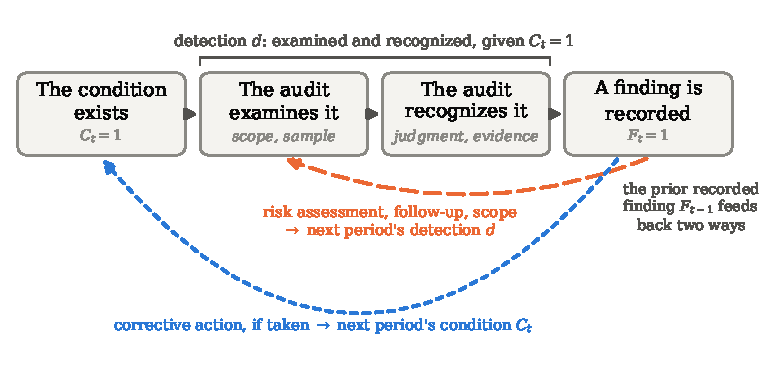
\includegraphics[width=\textwidth]{ex1_diagram.pdf}
\caption{\textbf{A finding history is also an observation history.} A recorded
finding ($F_t = 1$) requires the condition to exist ($C_t = 1$), the audit to
examine the area where it is, and the auditor to recognize it there. The
detection probability $d$ covers both steps together, given that the
condition exists: selection into observation as well as recognition.
The absence of a recorded finding is therefore three different things wearing
the same clothes: the condition was not there, or it was never looked for, or
it was looked for and missed. The two feedback arrows are what make the
record hard to read. The prior recorded finding $F_{t-1}$ feeds back two
ways: through corrective action, if any is taken, into next period's
condition $C_t$, and
through next period's risk assessment, follow-up plan and scope into next
period's detection probability $d$. Equation~\eqref{eq:long} is this diagram
written as a product, with $F_{t-1}$ inside both factors. In the Single Audit the feedback is written into the regulation rather
than inferred from behavior (Section~\ref{sec:regime}).}
\label{fig:diagram}
\end{figure}

\section{THREE PROGRAMS, ONE FINDING HISTORY}\label{sec:worlds}

Consider three programs. In each, the finding record shows the pattern
auditors recognize: a program with no finding last year has
about a \nWorldQzero{} chance of a recorded finding this year, and a program
with a finding last year has about a \nWorldQone{} chance. In the notation of
equation~\eqref{eq:qrd}, $q_0 = \nWorldQzero{}$ and $q_1 = \nWorldQone{}$.
Recorded findings are four times as likely after a finding year as after a
clean year. Any audit shop would read that as a strong predictor of another
recorded finding, and would reasonably plan accordingly.

Underneath, the three programs have nothing in common. Table~\ref{tab:worlds}
sets them side by side.

In the first, the condition really did persist. The chance the deficiency is
present rises from $r_0 = 0.100$ after a clean year to $r_1 = 0.400$ after a
finding year, and the audit catches half of what is there in both cases,
$d_0 = d_1 = 0.500$. Multiply: 0.100 times 0.500 is \nWorldQzero{}, and 0.400
times 0.500 is \nWorldQone{}. Equal detection halves the absolute rates and
their difference (a recorded gap of 0.15 against an underlying gap of 0.30)
and leaves the risk ratio exactly as it is underneath.

In the second, nothing about the condition changed at all. The deficiency is
present $r_0 = r_1 = 0.200$ of the time regardless of last year. What changed
is the looking. After a clean year the auditor catches $d_0 = \nWorldOdZero{}$
of what is there; after a finding year, under a follow-up requirement, the
auditor catches all of it, $d_1 = \nWorldOdOne{}$. Multiply: 0.200 times
\nWorldOdZero{} is \nWorldQzero{}, and 0.200 times \nWorldOdOne{} is
\nWorldQone{}. Identical record. The entire fourfold elevation is the
follow-up, and the prior finding carries no information about whether the
condition is there this year.

The third case is the one worth sitting with. Here remediation is stipulated
to halve the underlying rate: the chance the deficiency is present
\emph{falls} from $r_0 = 0.400$ after a clean year to $r_1 = 0.200$ after a
finding year. But the follow-up is thorough. Detection went
from $d_0 = 0.125$ to $d_1 = \nWorldOdOne{}$, a factor of \nWorldRdetRatio{}.
Multiply again and you get \nWorldQzero{} and \nWorldQone{}, the same two
numbers. In the record, programs coming off a finding year look four times
worse than programs coming off a clean year, and in this third case it is the
finding-year programs whose underlying rate is half as high. This column is
a constructed world compatible with successful remediation. It is not evidence
that remediation caused any decline; it shows that the record cannot rule the
possibility out.

The arithmetic is exact, and the three cases are three points on a continuum
along which the observed record is constant.

\subsection*{The observed ratio is a product}

The comparison auditors actually make is a ratio: how much more often findings
are recorded after a prior finding than after a clean year. Three ratios are
needed to say what that comparison contains.

$\Robs = q_1/q_0$ is the \emph{observed finding risk ratio}: how much more
often findings are recorded after a prior finding. In Table~\ref{tab:worlds}
it is 4 in every column, and it is the only one of the three the record
reports.

$\Rlat = r_1/r_0$ is the \emph{underlying-condition risk ratio}: how much
more often the problem itself exists after a prior finding. It is what a
planner would like to know.

$M = d_1/d_0$ is the \emph{history-conditioned detection multiplier}: how
much more likely an existing problem is to be detected in the prior-finding
group than in the clean-history group. Follow-up is the audit mechanism that
motivates it, and the paper calls it the follow-up detection multiplier for
short. It is a ratio of two detection probabilities, not a measure of hours,
sample size or effort.

All three ratios compare groups defined by prior recorded history. None of
them is a before-and-after effect of remediation or of follow-up on a given
program.

Dividing $q_1 = r_1 d_1$ by $q_0 = r_0 d_0$ gives
%
\begin{equation}\label{eq:product}
  \Robs \;=\; \Rlat \,\times\, M .
\end{equation}
%
The ratio of recorded finding rates is the product of the ratio of
underlying-condition rates and the ratio of detection probabilities. The
fourfold finding ratio in Table~\ref{tab:worlds} can come from a fourfold
ratio in underlying problems, a fourfold ratio in detection, or any
combination whose product is four. The table's last three
rows show the three cases: in Persistence, $\Rlat = 4$ and $M = 1$; in
Follow-up only, $\Rlat = 1$ and $M = 4$; in Remediation, $\Rlat = 0.5$ and
$M = 8$. Each multiplies to $\Robs = 4$. A fourfold finding ratio does not by
itself establish fourfold underlying risk, and it does not establish that
follow-up is working either. More years of the same kind of data do not help,
because every additional year is generated by the same product.

\subsection*{Successful remediation can raise recorded findings}

One corollary has a direct operational consequence. Suppose the underlying
condition is \emph{less} common in the prior-finding group, $r_1 < r_0$, as
successful remediation would make it. Recorded
findings still rise after a finding whenever
%
\begin{equation}\label{eq:reversal}
  M \;>\; r_0 / r_1 ,
\end{equation}
%
that is, whenever the follow-up detection multiplier exceeds the factor by
which the problem was reduced. If remediation halves the true problem rate but
follow-up makes detection more than twice as likely, the finding record rises
even though the underlying condition improves. In the Remediation column,
$r_0/r_1 = 2$ and $M = \nWorldRdetRatio{}$, and eight exceeds two. An
organization that judges its corrective-action process by comparing recorded
findings across history groups is using a comparison that can run the wrong
way precisely when the corrective action works and the follow-up is diligent
(Proposition~\ref{prop:remed}).

\begin{table}[tbp]
\centering
\caption{Three programs that produce exactly the same finding record.}
\label{tab:worlds}
\small
\begin{tabular}{lccc}
\toprule
& Persistence & Follow-up only & Remediation \\
\midrule
\multicolumn{4}{l}{\emph{Chance the condition is there, $r$\dots}} \\
\quad after a clean year, $r_0$ & 0.100 & 0.200 & 0.400 \\
\quad after a finding year, $r_1$ & 0.400 & 0.200 & 0.200 \\
\addlinespace
\multicolumn{4}{l}{\emph{Chance the audit detects it if it is there, $d$\dots}} \\
\quad after a clean year, $d_0$ & 0.500 & 0.250 & 0.125 \\
\quad after a finding year, $d_1$ & 0.500 & 1.000 & 1.000 \\
\addlinespace
\multicolumn{4}{l}{\emph{What the record shows, $q = r \times d$\dots}} \\
\quad after a clean year, $q_0$ & 0.05 & 0.05 & 0.05 \\
\quad after a finding year, $q_1$ & 0.20 & 0.20 & 0.20 \\
\addlinespace
\textbf{Observed finding risk ratio}, $R_{\mathrm{obs}} = q_1/q_0$ & \textbf{4.0} & \textbf{4.0} & \textbf{4.0} \\
\textbf{Underlying-condition risk ratio}, $R_{\mathrm{lat}} = r_1/r_0$ & \textbf{4.0} & \textbf{1.0} & \textbf{0.5} \\
\textbf{Detection multiplier}, $M = d_1/d_0$ & \textbf{1.0} & \textbf{4.0} & \textbf{8.0} \\
\bottomrule
\end{tabular}
\tablenotes{Read down each column. In all three, a program with no finding last year has a
5~percent chance of a recorded finding this year and a program with a finding
last year has a 20~percent chance, so the observed finding risk ratio
$R_{\mathrm{obs}}$ is 4 in every column. Underneath, the first program's
condition persisted, the second program's condition was no more likely than
before and only the looking changed, and in the third the underlying rate is
stipulated to be \emph{half} as high after a finding year while detection is
eight times as high. In each column the observed ratio is the product of the
underlying-condition ratio $R_{\mathrm{lat}}$ and the history-conditioned
detection multiplier $M$: $4 = 4 \times 1$,
$4 = 1 \times 4$, $4 = 0.5 \times 8$. Exact arithmetic, not simulation.}
\end{table}


\section[WHAT THE RECORD IDENTIFIES, AND WHAT IT ONLY BOUNDS]{WHAT THE RECORD IDENTIFIES,\\ AND WHAT IT ONLY BOUNDS}\label{sec:bounds}

The finding record does not point-identify the underlying condition, but it
does impose useful bounds. Three statements hold, needing in turn no
additional assumption about detection, one assumption about the direction of
follow-up, and one number about its size. All three rest on the
no-false-positive assumption of Section~\ref{sec:intro}.

\subsection*{With no additional assumption about detection: a floor and a wide range}

Because detection cannot exceed 100 percent, the true problem rate in each
history group must be at least as high as the recorded finding rate: $d_f \le
1$ in equation~\eqref{eq:qrd} gives $r_f \ge q_f$. If five percent of
clean-history program-years record a finding, at least five percent had the
condition. Without known complete detection, a recorded finding rate is a lower bound
on the underlying condition rate, not an estimate of it.

The question a planner asks is about the ratio, and the floor alone leaves it
wide. $\Rlat$ is largest when the prior-finding group's problem rate is as
high as possible (one) and the clean group's is as low as the record allows
($q_0$), and smallest in the reverse case, so
%
\begin{equation}\label{eq:unres}
  \Rlat \;\in\; [\,q_1,\; 1/q_0\,] ,
\end{equation}
%
and both ends can actually occur (Proposition~\ref{prop:bounds}). At the
values in Table~\ref{tab:worlds}, $q_0 = \nWorldQzero{}$ and $q_1 =
\nWorldQone{}$, so $\Rlat$ can range from $\nWorldQone{}$ to $20$. The same
fourfold recorded ratio is consistent with the underlying condition being five
times less common, equally common, or much more common after a prior finding.
Without information about detection, the record does not even fix the sign of
the underlying association.

\subsection*{With one assumption: the observed ratio is a ceiling}

Now assume that follow-up never makes the auditor look \emph{less} hard at a
program that had a finding than at one that did not: an existing problem is at
least as likely to be detected after a prior finding as after a clean history,
%
\[
  d_1 \;\ge\; d_0 , \qquad \text{equivalently } M \ge 1 .
\]
%
Call this monotone detection. The direction is consistent with a follow-up
regime, which directs more attention toward prior findings and never less,
but monotone detection remains a substantive assumption about how follow-up
affects the probability of detecting an existing condition, not a fact the
regulation proves; it fails, for example, when a prior finding shifts
attention toward one area and away from another, and it may hold for some
kinds of condition and not others.

Under monotone detection, dividing equation~\eqref{eq:product} by $M \ge 1$
gives
%
\begin{equation}\label{eq:mono}
  \Rlat \;\le\; \Robs .
\end{equation}
%
If follow-up can only increase detection, the recorded risk ratio cannot be
smaller than the underlying risk ratio. In Table~\ref{tab:worlds}, the underlying ratio is at most 4 in every
column, and the columns show it taking the values 4, 1 and 0.5. One
consequence needs no further information: if the recorded ratio is below one,
so that programs with a prior finding record \emph{fewer} findings than
programs without, the underlying association is genuinely negative, and no
amount of differential follow-up can explain it away.

\subsection*{With one number: a floor on the underlying ratio}

The constructive result comes from putting a ceiling on the follow-up
detection multiplier. Write $\Mbar$ for the largest value of $M$ the
organization is prepared to defend: the most that follow-up could plausibly
raise the chance of detecting an existing problem. If $1 \le M \le \Mbar$,
dividing equation~\eqref{eq:product} by $M \le \Mbar$ gives
%
\begin{equation}\label{eq:mbar}
  \Rlat \;\ge\; \Robs / \Mbar .
\end{equation}
%
Even after giving follow-up the largest detection advantage the organization
considers plausible, the underlying condition is still at least $\Robs/\Mbar$
times as common after a prior finding. A recorded ratio of 4 and a defensible
belief that follow-up can increase detection by no more than a factor of 2
implies an underlying risk ratio of at least 2. With equation~\eqref{eq:mono},
the record then places $\Rlat$ between 2 and 4: the inference survives, cut
down by the part of the elevation the follow-up can account for. And whenever
the recorded ratio exceeds $\Mbar$, the underlying association is genuinely
positive (Proposition~\ref{prop:mono}).

These bounds are sharp once the floor $r_f \ge q_f$ is added. Each detection
probability lies between $q_f$ and one, so the multiplier cannot exceed
$1/q_0$, and the multipliers consistent with the record are $1 \le M \le
\min\{\Mbar, 1/q_0\}$. The identified set is
%
\begin{equation}\label{eq:sharp}
  \Rlat \;\in\; \Bigl[\, \max\Bigl\{ q_1,\; \frac{\Robs}{\Mbar} \Bigr\},\; \Robs \,\Bigr] ,
\end{equation}
%
and every value in it is produced by some admissible pair of detection
probabilities (Proposition~\ref{prop:mono}(iii)). At the values of
Table~\ref{tab:worlds} with $\Mbar = 2$ the set is $[2, 4]$.

The binding identification constraint on what an auditor can learn from a
finding record is therefore not sample size or a more elaborate estimator; it
is what can be said about detection, summarized in $M$. Sample size still
governs precision. The propositions are population statements about $q_0$ and
$q_1$; in data, $\Robs$ is estimated, and each conclusion needs the matching
confidence limit. A negative underlying association requires an upper
confidence limit for $\Robs$ below one. A positive association under a
defended $\Mbar$ requires a lower confidence limit for $\Robs$ above
$\Mbar$. What can be said about detection is a question about audit
procedures, answerable by the organization that performs them and not from
the record; Section~\ref{sec:operational} sets out how.

\subsection*{More years of history do not remove the problem}

A longer record does not solve this on its own. Take any recorded history of
any length and any story about how likely the underlying problem was at each
point, so long as it stays at or above the recorded rate. Setting detection
at each point to whatever value reconciles the two reproduces the entire
recorded history exactly (Proposition~\ref{prop:full}). Adding years adds observations of the product
$q = rd$, not of either factor. Restricted models of the underlying condition
can nevertheless be identifiable when substantive restrictions constrain how
the condition evolves and how detection responds to the record
\citep{allman2009}; identification then comes from those restrictions, not
from record length alone. This paper does not estimate such a model. Its
interest is what can be said before those restrictions are imposed, and what
audit design can add.

\section{The Single Audit as a history-dependent observation regime}\label{sec:regime}

The empirical illustration comes from the Single Audit, and its terms need
defining before the data are read.

A Single Audit is an organization-wide audit required of nonfederal entities,
such as states, local governments, universities and nonprofits, that expend
federal awards above a regulatory threshold. It combines a financial statement
audit with compliance testing of the entity's federal programs, and its
structured results are published by the Federal Audit Clearinghouse.

Compliance testing is not spread evenly across every program. The auditor
designates certain federal programs as \emph{major programs} and performs the
required major-program compliance audit on them. Programs not selected as
major do not receive that full program audit solely by virtue of program
status, although other work, including required follow-up of prior findings,
may still occur. The selection is risk based. Programs whose federal
expenditures exceed the Type~A threshold are \emph{Type~A}; the rest are
Type~B. The threshold is tiered by the entity's total federal expenditures:
over the sample period it was \$750,000 for entities expending up to \$25
million and higher in tiers above that (2~CFR 200.518(b)(1)). A Type~A program that meets a list of low-risk criteria may be
left out of detailed testing in a given year, and one that fails the criteria
must be tested as major. Prior findings are among
the criteria: a material weakness, a modified opinion on the program, or
questioned costs above five percent of the program's expenditures in the most
recent audit period disqualify a Type~A program from low-risk
treatment.\footnote{Not every prior finding does this. A significant
deficiency that is not a material weakness, or questioned costs below the
five-percent line, leaves a Type~A program eligible for low-risk treatment.
The paper does not assume that every prior finding makes major-program
coverage more likely, and its sample construction conditions on major-program
coverage in both years.} The
requirements tested for a major program are those the Office of Management and
Budget's annual \emph{Compliance Supplement} designates as applicable to it.

Separately, and regardless of program selection, the auditor must follow up on
prior audit findings, whether or not the program with the prior finding is
selected as major again. In the governing regulation, prior findings raise
assessed program risk (2~CFR 200.519(b)(2)); they can disqualify a Type~A
program from low-risk treatment (200.518(c)(1)); and follow-up is mandatory
``regardless of whether a prior audit finding relates to a major program in
the current year'' (200.514(e)). None of this is a defect; the follow-up requirement exists
because findings left uncorrected are a documented problem in this program
\citep{gao2002}.

The setting is useful for one reason. In most inspection systems the feedback
from past results to present attention has to be inferred from inspector
behavior. Here it is written into the rules, through two channels: a coverage
channel, in which a prior finding can change whether a program is tested in
depth at all, and a condition-specific channel, in which a prior finding must
be followed up wherever it sits. Restricting the sample to programs audited as
major in both years conditions on the major-program-selection channel: every
comparison is among programs selected in both years. That conditioning does
not make the selection ignorable, and it does not hold audit intensity or
condition-specific observation fixed: the
follow-up channel is mandated inside the restricted sample, so two such
programs, one with a prior finding and one without, face different
condition-specific attention by regulation even though both are audited in
depth in both years.

\section{FAC EVIDENCE: RECURRENCE, NEW FINDINGS, AND MIXED CASES}\label{sec:fac}

Prior work has established that Single Audit findings recur and that a
reported finding depends jointly on the condition existing and on the auditor
detecting it
\citep{keating2005,petrovits2011,waymire2018,gao2002,gao2024,waddell2023}.
What is added is the decomposition of what follows a prior finding into
recurrence, newly recorded findings and mixed cases.

\subsection*{Data and sample}

The data are the public Federal Audit Clearinghouse bulk files; the unit of
analysis is the auditee--program--year, and the window is fiscal years 2016
through 2023, inside a single audit-threshold regime \citep{omb2024}. Of
\nPanelRows{} program-years, \nResolvedRows{} have a resolved prior-year
observation of the same program, and Sample~A restricts further to the
\nSampleA{} in which the program was audited as a major program in both
years: \nNPrior{} with a prior-year finding and \nNNoPrior{} without.
Intervals are cluster bootstrap over \nNAuditees{} auditees.
Appendix~\ref{app:emp} gives the construction and the sample flow.

One construction decision follows from the paper's own argument. In
\nSthreeN{} program-years, \nSthreePct{} percent of the panel, the auditee
filed in the prior year but this program does not appear in that filing. They
are excluded rather than coded as ``no prior finding'', because the absence of
a record is not a clean result: they go on to record a finding
\nSthreePctFinding{} percent of the time, against \nStwoPctFinding{} percent
after a resolved clean prior year. ``Repeat'' is the auditor's own coding; a
validated historical link is the secondary definition
(Appendix~\ref{app:emp}).

\subsection*{What follows a prior finding}

Even among programs audited as major in both consecutive years, prior recorded
findings predict two distinct parts of the future finding record: explicit
recurrence, and additional newly recorded findings. Table~\ref{tab:fourstate}
is the main result. For context, a program-year following a clean prior year
records a finding \mPAnyNoPrior{} of the time and one following a prior-year
finding records one \mPAnyPrior{} of the time, a difference of \mDAny{}
$[\mDAnyLo{},\,\mDAnyHi{}]$ and a ratio of \nRRAny{}. The content is in
how that difference is made up.

A program-year lands in exactly one of four states: no finding ($0$); a repeat
finding and nothing else ($R$); a new finding and nothing else ($N$); or both
a repeat and a new finding ($B$). Write $\Delta$ for the difference in the
probability of a state between program-years with and without a prior
finding. Because the four states do not overlap and cover every possibility,
the differences add:
%
\begin{equation}\label{eq:four}
  \Delta_{\text{any finding}}
  \;=\;
  \Delta_{R}
  \;+\;
  \Delta_{N}
  \;+\;
  \Delta_{B} .
\end{equation}
%
The categories can be added without deciding where mixed cases belong,
because each mixed case is counted once, in $B$. In Sample~A, $\Delta_R =
+\nDRonly{}$, $\Delta_N = +\nDNonly{}$ and $\Delta_B = +\nDBoth{}$, adding to
$+\nDAny{}$. Every interval in the table excludes zero.

Most of the gap is repeat-involving, as an auditor would expect. The row that
is easy to read past is the one about new findings. Programs whose \emph{only}
outcome was a new finding account for $+\nDNonly{}$, a ratio of \nRRNonly{},
which looks like almost nothing. But ``new only'' does not answer the
question a reader is asking, which is whether the program recorded \emph{any}
newly recorded problem. That quantity is
%
\[
  \text{any new} \;=\; N + B ,
\]
%
because a period that recorded both a repeat and something new did record
something new. On that margin the difference is $+\nDAnyNew{}$
$[\nDAnyNewLo{},\,\nDAnyNewHi{}]$, from \mPAnyNewNoPrior{} to
\mPAnyNewPrior{}, a ratio of \nRRAnyNew{}. The two ratios, \nRRNonly{} and
\nRRAnyNew{}, differ by a factor of \nRRfactor{} and come from the same table.
The difference between them is definitional, not evidence about follow-up:
``new only'' excludes every period that also recorded a repeat, and ``any
new'' includes them. Periods land in $B$ for more than one reason, and these
data do not separate them: thorough follow-up of a repeat can put a program
there that would otherwise have shown only a new finding, and so can a program
simply having several distinct deficiencies.

The cleanest version counts findings rather than flagging programs. Every
individual finding is classified once, as a repeat or as new, so the
difference in the expected number of findings splits with no allocation rule
at all:
%
\begin{equation}\label{eq:count}
  \underbrace{+\nEtotal{}}_{\text{total}}
  \;=\;
  \underbrace{+\nErepeat{}}_{\text{repeat}}
  \;+\;
  \underbrace{+\nEnew{}}_{\text{new}} .
\end{equation}
%
A program-year following a prior-year finding records about one more finding
than one following a clean year, of which roughly seven tenths of a finding
is a repeat and three tenths is new.

The record does not identify how much of these associations reflects true
persistence of the underlying condition, stable differences between auditees,
condition-specific follow-up, broader scrutiny of programs with a history,
remediation combined with heavier detection, or mixtures of these. Each is
consistent with Table~\ref{tab:fourstate}. The FAC results illustrate the
identification problem; they do not identify its mechanism, and nothing here
should be cited as showing that observation feedback is the dominant
explanation.

\subsection*{A recurrence share is a convention, not a measurement}

The obvious way to compress Table~\ref{tab:fourstate} into one number is to
ask what share of the prior-finding association is recurrence. That statistic
is not uniquely defined when a program-period can contain both repeat and new
findings, because every mixed period, \nMixedShare{} percent of all
prior-finding outcomes, has to be assigned to one side. Assign none of them to
recurrence and the share is \nZetaLo{} percent. Assign all of them and it is
\nZetaHi{} percent. The summary moves \nZetaSwing{} percentage points, and
nothing in the underlying observations changes (Figure~\ref{fig:zeta}). The
general lesson: when outcome classes overlap, report mutually exclusive states
or additive counts before reporting an attributable share, and if a share is
reported anyway, state the convention and show the figure under the opposite
one. The convention-free statement is equation~\eqref{eq:four}:
$\nDAny{} = \nDRonly{} + \nDNonly{} + \nDBoth{}$.

\subsection*{A comparison the data do not support}

A natural next question is whether prior findings predict problems in
requirement areas that never had one. The Clearinghouse records the
requirement category attached to every reported finding. It does not record
the universe of requirements that applied to, and were tested in, each
program-year; that universe is defined by the Compliance Supplement and is
external to these data. A ``first finding in a previously clean area'' rate
therefore has no defensible denominator, and without one the comparison goes
wrong because the two history groups do not have the same opportunity to
produce the outcome. Take two requirement areas, each with a 0.20 chance of a
finding this year, independent of anything before. A program with neither
area previously flagged has a $1 - 0.80^2 = 0.36$ chance of a finding in an
area new to it; a program with one area already flagged has only the other
available, so its chance is $0.20$. Nothing underneath differs. In a
constructed twelve-area case in which nothing depends on history, the naive
new-area risk ratio is \mNullCategoryRR{}: prior-finding programs look about
thirty percent \emph{less} likely to have a new kind of problem, from unequal
opportunity alone. No denominator was invented, and the comparison is not
made.

\subsection*{Robustness}

Table~\ref{tab:specs} in Appendix~\ref{app:emp} reports every specification.
Restricting to transitions with stable Clearinghouse provenance moves the
any-finding gap from \nDAny{} to \nProvDeltaAny{} and leaves any-new at
\nProvDeltaAnyNew{}. Substituting the validated historical link for the
auditor's repeat flag moves the repeat-only gap to \nVlinkDeltaRonly{} and
the both-kinds gap to \nVlinkDeltaBoth{}, leaves any-new unchanged, and opens
a fifth outcome state worth \nVlinkFifth{} of the gap, given its own column
there. A prespecified three-year history rule, under which ``no prior
finding'' means three observed clean years, leaves \nHtwoSampleA{}
program-years and attenuates the gaps to \nHtwoDeltaAny{} for any finding and
\nHtwoDeltaAnyNew{} for any new. Across all five specifications the any-new
margin moves least.

\begin{table}[tbp]
\centering
\caption{What follows a prior-year finding.}
\label{tab:fourstate}
\footnotesize
\setlength{\tabcolsep}{4.5pt}
\begin{tabular}{lccccr}
\toprule
& \multicolumn{2}{c}{Chance this year} & & & \\
\cmidrule(lr){2-3}
Outcome for the program-year & \shortstack{no prior\\finding} & \shortstack{prior\\finding}
& Difference & 95\% interval & Ratio \\
\midrule
No finding at all & 0.9234 & 0.4217 & $-0.5017$ & $[-0.5104,\, -0.4927]$ & 0.46 \\
A repeat finding only & 0.0015 & 0.3088 & $+0.3073$ & $[0.3008,\, 0.3140]$ & --- \\
A new finding only & 0.0744 & 0.1200 & $+0.0456$ & $[0.0416,\, 0.0498]$ & 1.61 \\
Both a repeat and a new finding & 0.0007 & 0.1495 & $+0.1488$ & $[0.1416,\, 0.1561]$ & --- \\
\midrule
Any finding & 0.0766 & 0.5783 & $+0.5017$ & $[0.4927,\, 0.5104]$ & 7.55 \\
Any repeat finding & 0.0022 & 0.4583 & $+0.4561$ & $[0.4458,\, 0.4656]$ & --- \\
\textbf{Any new finding} (new only $+$ both) & 0.0751 & 0.2696 & $+0.1945$ & $[0.1870,\, 0.2021]$ & 3.59 \\
\midrule
\multicolumn{6}{l}{\emph{Findings counted rather than programs flagged --- this needs no allocation rule:}} \\
Findings recorded, total & 0.1029 & 1.1712 & $+1.0683$ & $[1.0209,\, 1.1182]$ & \\
\quad of which repeat & 0.0027 & 0.7468 & $+0.7441$ & $[0.7084,\, 0.7807]$ & \\
\quad of which new & 0.1002 & 0.4245 & $+0.3243$ & $[0.3076,\, 0.3422]$ & \\
\bottomrule
\end{tabular}
\tablenotes{Sample A: 206,926 program-years
in which the same program was audited as a major program in both years, 39,067 with
a finding in the prior year and 167,859 without. The four outcomes in the first panel
are mutually exclusive and, under the auditor's repeat flag used here, exhaust
the possibilities, so their risk differences add to the difference in ``any
finding'' exactly. Intervals are 95 percent
cluster bootstrap, 1,000 replications resampling 45,952 auditees with their full
histories, seed 20260918. Every interval excludes zero. The row that is easy to miss
is ``any new finding'': counting only the periods whose \emph{sole} outcome was
new understates it by roughly a factor of 2.23 on the ratio scale, because ``new
only'' excludes every period that also recorded a repeat. A period can land in
``both'' because repeat follow-up is thorough, or because the program has
several distinct deficiencies; these data do not separate the two. The
ratio column is left blank for the three repeat-involving rows.
Repeat-involving baseline probabilities are very small in this sample, making
their ratios sensitive to small denominators; risk differences are reported
instead.}
\end{table}


\begin{figure}[tbp]
\centering
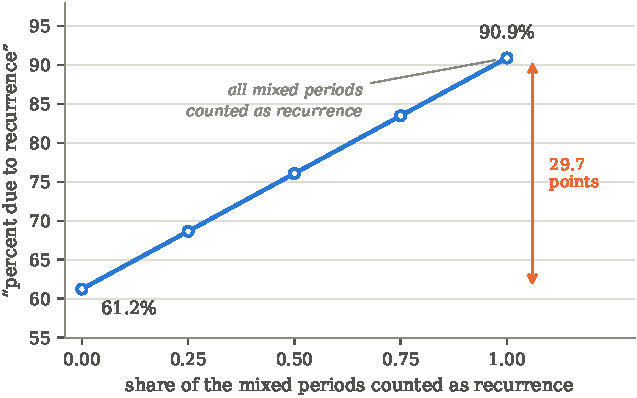
\includegraphics[width=0.78\textwidth]{ex7_zeta.pdf}
\caption{\capZeta}
\label{fig:zeta}
\end{figure}

\section{FOLLOW-UP AND DISCOVERY}\label{sec:design}

Auditors already have the vocabulary for the distinction the results point
at. Follow-up is returning to a previously identified problem. Discovery is
learning where problems exist outside what has already been identified. Both
are part of the work, and they are not the same job.

For follow-up, a record of prior findings is close to ideal routing
information: it identifies the known conditions that deserve revisiting, and
the regulation is right to require the visit. It is not sufficient
verification that a condition remains; the follow-up procedures generate that evidence, and the
Single Audit results are consistent with follow-up working as designed.
Discovery concerns conditions not already represented in the finding history.
Prior findings can carry genuine information about it: some entities are
durably more susceptible across the board, and one underlying weakness can
produce several kinds of condition. What the record cannot say is how much of
that apparent signal is susceptibility and how much is the observation
process, because the places without findings are precisely where absence and
non-detection cannot be separated, and because a prior finding can widen the
search. A record built by looking where the record said to look contains
information about the places that were looked at; how much it contains about
everywhere else is the question it cannot answer about itself.

The distinction has a testable shape, because different audit responses to a
prior finding leave different marks on the outcomes of
Table~\ref{tab:fourstate}. Table~\ref{tab:multitype} works through three ways
an auditor might let last year's finding change this year's work, with the
underlying problems held identical and drawn independently each period, so
nothing underneath persists at all. Every cell is the change in the
prior-finding gap relative to a baseline in which prior findings change
nothing. The regimes share their first-period histories, so the history
groups and each program's previously flagged conditions and areas are the
same in every regime; they share second-period conditions and detection draws
program by program; and each regime changes detection only for the conditions
it targets. An outcome outside a regime's target set is therefore identical,
program by program, to its baseline value, which makes the zeros exact and
cancels the opportunity-set artifact of Section~\ref{sec:fac}. New findings are
separated by whether they fall in a requirement area that already had one,
because that is where the three responses part company.

\emph{Condition-specific follow-up.} If the response is to re-test the control
or re-examine the transactions behind the specific finding, repeat findings
rise and nothing else moves; the two new-finding outcomes are exactly zero.

\emph{Category-level follow-up.} If the response is to tighten work across the
whole requirement area that produced the finding, repeats rise and so do new
findings inside that area, while areas never flagged remain untouched.

\emph{Generalized scrutiny.} If the response is general wariness, so that a
program with a finding simply gets a harder audit everywhere, all three
outcomes move, including findings in requirement areas that never had one.
That last column is the one to watch, because a finding in a previously clean
area is exactly what an auditor would read as a genuinely new and independent
problem.

A new finding is therefore not automatically independent evidence of a new
underlying problem, because a prior finding may have changed how broadly the
auditor searched. The converse holds with equal force: broadly elevated
findings are also consistent with programs that are genuinely worse across the
board, and with stable differences between auditees that make some of them
durably more prone to deficiencies (Appendix~\ref{app:id}). The table narrows the space of explanations; it does not identify the
mechanism. In the Clearinghouse data the elevation runs across repeat-only,
mixed and any-new outcomes, which is the pattern the last two rows of
Table~\ref{tab:multitype} produce and the pattern a worse program produces,
and the record cannot say which.

The design question that follows is not how to squeeze more out of the
finding record but what additional information would separate the two factors
in equation~\eqref{eq:qrd}. Section~\ref{sec:scoring} shows what happens when
that question is skipped; Section~\ref{sec:operational} answers it.

\begin{table}[tbp]
\centering
\caption{\textbf{How you look decides what turns up.} Three ways of letting last
year's finding change this year's audit, with the underlying problems held
identical and drawn independently each period. Each cell is the change in the
gap between programs with and without a prior finding, measured against a
baseline in which prior findings change nothing. Following up the same finding
moves repeats and \emph{only} repeats. Looking harder across a requirement area
also surfaces new findings inside that area. Looking harder at the program
overall also surfaces findings in areas that never had one --- which is what an
auditor would otherwise read as a genuinely new problem. The zeros are exact:
they come from using the same random draws across regimes.}
\label{tab:multitype}
\small
\begin{tabular}{lccc}
\toprule
& \multicolumn{3}{c}{Change in the prior-finding gap} \\
\cmidrule(lr){2-4}
If last year's finding makes the auditor\dots
& \shortstack{A finding\\repeats}
& \shortstack{Something new,\\in an area that\\already had one}
& \shortstack{Something new,\\in an area that\\did not} \\
\midrule
Follow up the same finding & $+0.0394$ & $+0.0000$ & $+0.0000$ \\
Look harder at the same requirement area & $+0.0279$ & $+0.0454$ & $+0.0000$ \\
Look harder at the program overall & $+0.0223$ & $+0.0366$ & $+0.1388$ \\
\bottomrule
\end{tabular}
\end{table}


\section{RISK MODELS TRAINED ON FINDING HISTORIES}\label{sec:scoring}

Audit organizations increasingly build models that score programs for risk and
validate them the way any predictive model is validated: fit on one period,
test on another, report an AUC, check calibration. The metrics are not broken.
They answer a precise question about the label they are given, and the label
is the recorded finding. The error is to carry the result over and describe
the model as predicting where problems are. It has teeth because a score that
steers where auditors look can make itself right: a flagged program gets more
attention, more attention raises detection, higher detection produces recorded
findings, and the recorded findings validate the score
\citep{ensign2018,lum2016,lakkaraju2017,kleinberg2018}. The obvious objection
is that this is just a story about auditing more, so the construction worth
making holds average detection fixed.

Figure~\ref{fig:budget} does that. Across the whole horizontal axis the
average chance of catching an existing condition stays at
\mBudgetDetection{} and the overall recorded finding rate stays at
\mBudgetPrevalence{}. The only thing that changes is allocation: detection
moves away from the programs the score does not flag and toward the programs
it does. The score is statistically independent of where the conditions
actually are; it knows nothing. Measured against the recorded finding, its
AUC climbs from \mBudgetAucFstart{}, a coin flip, to \mBudgetAucFend{}, and
its Brier score improves. Measured against the underlying condition, its AUC
is exactly \mBudgetAucC{} at every point and its Brier score worsens by exactly
the amount the recorded-label Brier score improves.
On a validation report this reads as a model that became genuinely
discriminating, with no change in average detection. The calculation is
exact, from a single prespecified configuration.
Appendix~\ref{app:pred} gives the grid, the general result, a fitted rather
than an oracle score, and the finite-sample distributions at portfolio sizes
an audit organization actually has. Calibration is no stronger a guarantee: a
model can be perfectly calibrated for recorded findings while carrying no
information about the underlying condition at any point of its range, and the
appendix works a case in which predictions span a factor of \nCalibSpan{}
across deciles while the underlying problem rate is flat in all ten.

The implication is narrow. Reporting that a risk model achieves a given AUC
against recorded findings is a true and useful statement and should be made
in exactly those words. An ordinary train/test split does not detect the
problem, because both halves were produced by the same audit process under
the same targeting policy. What cannot be concluded is that the model has
located where problems are; if the model also influences audit planning, the
validation evidence is partly a record of the model's own effect on the
audit.

\begin{figure}[tbp]
\centering
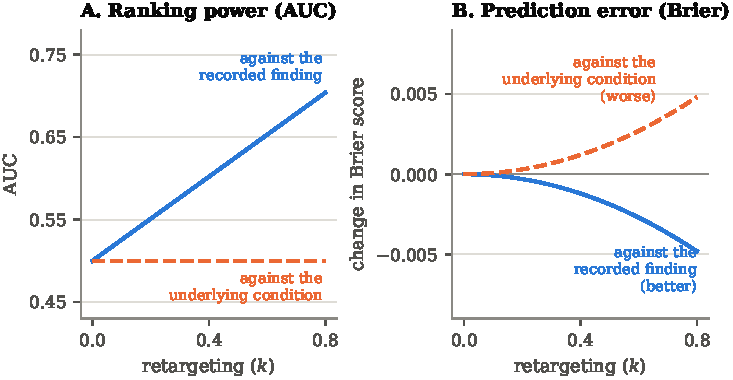
\includegraphics[width=0.85\textwidth]{ex3_fixed_budget.pdf}
\caption{\capFixedBudget}
\label{fig:budget}
\end{figure}

\section{MAKING THE BOUND OPERATIONAL: LEARNING ENOUGH ABOUT DETECTION TO USE IT}\label{sec:operational}

The bound in equation~\eqref{eq:mbar} does work only when the organization can
say something about $M$. Two things need to be clear about $M$ before any
route to it is described.

The first is what $M$ is not. $M = d_1/d_0$ is the ratio of two
probabilities: that an existing condition is detected after a prior finding,
and that it is detected after a clean history. It is not audit effort. Hours,
sample sizes, coverage percentages and procedure counts are not $M$, and
doubling any of them does not double $M$; they inform $M$ only through a
defensible connection to detection.

The second is that $M$ is target-specific. The multiplier is defined for a
particular detection target: a defined condition, finding class, procedure or
audit objective. Different compliance requirements, finding types, control
deficiencies and transaction tests can have different $d_0$, different $d_1$
and therefore different $M$. An organization should not assume that follow-up
has the same detection effect for every condition, requirement or procedure.
In practice the useful object is $M$ for a stated finding class, or a
defensible bound that applies to a specified family of conditions; the text
keeps the single symbol $M$ for readability, with that scope understood.

Six ways to learn or bound $M$ follow, each with different information
requirements and identifying assumptions. Table~\ref{tab:designs} summarizes
what each supplies and the assumption on which it turns.

\subsection*{Reference observation under a common measurement rule}

The cleanest design is reference observation under a common measurement rule:
a set of program-years in each history group, examined with the same
reference procedure, chosen so that the reference observations represent the
population whose condition rate is being estimated. The reference sample does
not have to ignore prior history. It may be stratified on prior-finding
status; what matters is that within each history group it represents that
group, through probability sampling or known weights. Tax administrations
maintain random examination programs beside operationally selected ones for
this reason \citep{slemrod2019}, and safety regulators have randomized
inspection allocation \citep{levine2012}.

Let $s$ be the sensitivity of the reference procedure for the target
condition, the probability it detects that condition when present. One extra
symbol is needed because the reference procedure is a different procedure
from the targeted audit, with its own detection probability, and $s$ is
unknown. If $s$ is the same in both history groups, the reference finding
rates are $q^{\mathrm{ref}}_0 = r_0\, s$ and $q^{\mathrm{ref}}_1 = r_1\, s$,
so
%
\begin{equation}\label{eq:ref}
  \frac{q^{\mathrm{ref}}_1}{q^{\mathrm{ref}}_0}
  \;=\;
  \frac{r_1\, s}{r_0\, s}
  \;=\;
  \Rlat .
\end{equation}
%
The reference procedure does not need perfect detection to recover the
underlying risk ratio. It needs the same sensitivity in both history groups,
because a common sensitivity cancels, and only then.
\begin{center}
\fbox{\parbox{0.9\textwidth}{\emph{A reference procedure does not need
perfect detection to identify the underlying risk ratio. It needs comparable
detection in the two history groups, and negligible false positives.}}}
\end{center}
With $\Rlat$ in hand, equation~\eqref{eq:product} gives the multiplier
directly:
%
\begin{equation}\label{eq:mfromref}
  M \;=\; \Robs / \Rlat .
\end{equation}
%
In words: the targeted audit gives the ratio of finding rates between the two
history groups. The reference work gives the ratio of underlying condition
rates, under a common measurement rule. Their ratio identifies the
multiplicative detection component $M$. If the targeted record shows the
fourfold ratio of Table~\ref{tab:worlds} and the reference sample shows
findings twice as often after a prior finding as after a clean year, then
$\Rlat = 2$ and $M = 4/2 = 2$: the observed fourfold ratio factorizes into a
twofold underlying-condition ratio and a twofold detection multiplier.
Section~\ref{sec:fac} could not do this because the Clearinghouse contains no
such sample.

Five assumptions carry the result (Proposition~\ref{prop:ref}). First, within
each prior-history group the reference sample represents the population whose
condition rate is being estimated, directly or through known sampling
weights. Second, the same reference measurement rule is applied in both
groups. Third, the reference procedure has common sensitivity across the two
groups for the target condition. Fourth, the reference observation does not
alter the condition before it is measured. Fifth, the reference procedure has
negligible false positives for the target condition, or its false-positive
process is separately modeled; a reference that records findings where no
condition exists does not cancel in the ratio. The third is the load-bearing
one,
and applying the same nominal procedure does not by itself guarantee it.
Sensitivity can differ between the groups if the conditions in one group are
more severe or of different types, if records are harder to obtain, if the
procedure is implemented differently, or if the case mix differs; then the
reference ratio is $\Rlat$ times the ratio of sensitivities and the
cancellation fails. Reference-sample size should be planned from the desired
precision and the expected condition or finding rates in the two history
groups.

\subsection*{High-sensitivity reference procedures}

A second anchor comes from procedures whose sensitivity for a narrowly defined
condition is known or credibly near-perfect. Where such a procedure is applied
to a whole subpopulation, its finding rate estimates that subpopulation's
condition rate, so $r$ is observed rather than bounded, and the targeted
procedure's finding rate in the same group then gives its detection
probability, $d = q/r$; anchors in both history groups yield $d_0$, $d_1$ and
$M$.

The anchor rests on the procedure's sensitivity, not on its coverage.
Exhaustive coverage by itself does not make detection perfect. It removes
sampling or coverage uncertainty, and it anchors the underlying rate only when
the procedure applied to that population has known or credibly near-perfect
sensitivity for the target condition. Where auditors speak of ``certainty
testing'', the certainty refers to inclusion in the tested population, not to
certainty that every existing condition will be recognized. Testing every
transaction for an exact duplicate payment may plausibly have very high
sensitivity for that narrowly defined condition; testing every file for a
judgment-dependent compliance failure may not, and the anchor is then only as
good as the sensitivity that can be defended.

\subsection*{Independent reference adjudication}

A representative or appropriately weighted sample of program-years within
each history group can be re-adjudicated by a reviewer who does not see the
original finding history and applies a fixed program of work. Blindness
removes the history's influence on the reviewer; it does not by itself create
ground truth, and two cases have to be kept apart.

In the first, a sufficiently accurate reference or adjudication procedure is
available for the target condition. Then the reference review approximates
latent status, $d_0$ and $d_1$ are estimated directly as the share of
reference-identified conditions the original audit had recorded in each
history group, and $M$ is their ratio; this is the audit analogue of
correcting a diagnostic study for differential verification
\citep{degroot2011}. In the second, the reference review is itself imperfect.
Then its own error process has to be addressed, through multiple independent
procedures, a model of detection that treats the reference as one more
imperfect measurement, or an external benchmark with known properties.
Ordinary blind re-performance of the same work does not automatically solve
the problem, because both reviews may miss the same condition for the same
reason, and the shared misses are invisible to both.

\subsection*{Two distinct detection procedures}

Two imperfect procedures can reveal how much each is missing. Suppose
procedure A vouches transaction-level evidence and procedure B obtains an
independent external confirmation or performs a genuinely different
control-based test, both applied to the same programs. Under conditional independence of the two procedures' failures and stable
sensitivity, and with no false positives, the share of the conditions B finds
that A also finds identifies A's detection probability; the share of the
conditions A finds that B also finds identifies B's; and the overlap then
says how many conditions both missed. This is the logic ecologists use to
estimate how often a species is present at sites where a survey did not see it
\citep{mackenzie2002}, and it needs no reference sample
(Proposition~\ref{prop:twoproc}).

Two requirements carry it. The procedures' failures must be unrelated once
the true condition is fixed, and each procedure's sensitivity must be stable
across the program-years being pooled. Using two operationally different
procedures is not enough on its own: if both tend to miss the same difficult
cases, for example where documentation does not exist, their agreement looks
reassuring while saying little about what both missed. Vouching paired with
an external confirmation can satisfy the first requirement; two reviewers
re-performing the same sample with the same method generally cannot.

\subsection*{Randomized or quasi-random changes in audit attention}

Some changes in how hard an audit looks arrive for reasons unrelated to the
underlying condition: randomized rotation, random reference selections,
externally imposed coverage rules, staffing changes plausibly unrelated to the
control environment, randomized review depth. These reveal how finding rates
change when observation changes. A change in audit attention is informative
about detection only if the change does not independently alter, or select
on, the underlying condition; that is the exclusion restriction, and a
staffing increase introduced because controls deteriorated fails it. And such
variation identifies relative detection effects between the regimes it
creates, or tightens bounds; absolute condition prevalence generally requires
an additional sensitivity anchor of the kind described above.

\subsection*{Procedure-based bounds}

An organization that can do none of the above may still be able to defend an
upper bound $\Mbar$ from what it knows about its own procedures: the fraction
of the population covered, sample sizes, the number and type of compliance
requirements tested, the use of targeted versus broad procedures, the strata
tested with a high-sensitivity procedure, historical quality-review results,
and any external validation study. These quantities are not $M$. They inform
$M$ only through an explicit model connecting audit procedures to detection
probability, for instance a statement of what share of existing conditions a
procedure of a given depth is expected to catch, and the bound is only as
defensible as that model.

The arithmetic once $\Mbar$ is in hand is simple. If the organization can
defend $M \le 1.5$ for the finding class in question and observes $\Robs =
3$, equation~\eqref{eq:mbar} gives $\Rlat \ge 3/1.5 = 2$: even after giving
follow-up the largest detection advantage the organization considers
defensible, the underlying condition must still be at least twice as common
in the prior-finding group, and with monotone detection the underlying ratio
lies between 2 and 3. What the record could only place between $q_1$ and
$1/q_0$ has become a range an audit committee can act on.

The remaining route is a structural model whose restrictions on how the
condition evolves and how detection responds are defended on audit grounds;
identification then has to be established for that specific model, and this
paper does not take that route.

\begin{table}[tbp]
\centering
\caption{\textbf{Six ways to learn or bound the follow-up detection
multiplier.} What each design supplies and the assumption on which it turns.
$M = d_1/d_0$ is defined for a stated condition, finding class or procedure;
the designs are not ranked, because they answer different questions with
different information requirements. Details and the remaining assumptions
for each are in Section~\ref{sec:operational}; the first two identifying
results are Propositions~\ref{prop:ref} and \ref{prop:twoproc} in
Appendix~\ref{app:id}.}
\label{tab:designs}
\small
\begin{tabular}{p{0.30\textwidth}p{0.30\textwidth}p{0.32\textwidth}}
\toprule
Design & What it supplies & Critical assumption \\
\midrule
Reference observation under a common measurement rule & $\Rlat$, hence $M = \Robs/\Rlat$ & Common sensitivity in the two history groups; no false positives \\
High-sensitivity reference procedure & Anchor for $r$, hence $d = q/r$ & Known or credibly near-perfect sensitivity for the target condition \\
Independent reference adjudication & $d_0$, $d_1$ directly & Reference status credible enough to stand in for the condition \\
Two distinct procedures & $r$, $d$ within a history group & Conditionally independent failures; stable sensitivity; no false positives \\
Randomized or quasi-random attention shift & Relative detection; tighter bounds & Exclusion restriction: the shift does not alter or select on the condition \\
Procedure-based bound & $\Mbar$, hence $\Rlat \ge \Robs/\Mbar$ & A defensible model linking procedures to detection probability \\
\bottomrule
\end{tabular}
\end{table}


\section{CONCLUSION AND BOUNDARIES}\label{sec:conclusion}

The paper set out to answer four questions.

\emph{What can the finding record tell us?} A finding history predicts the
future finding record. It fixes a floor under the underlying condition rate
in every history group and, if follow-up can only raise detection, a ceiling
on the underlying-condition risk ratio: the observed finding ratio. Where the
observed ratio is below one, the underlying association is negative.

\emph{What can it only bound?} The underlying-condition risk ratio itself.
Without information about detection, the record places it anywhere between
$q_1$ and $1/q_0$, an interval that at ordinary finding rates contains one and
runs well below it. A longer record does not narrow the interval, because
every added year is another observation of the product $q = rd$.

\emph{Why is follow-up different from discovery?} A prior finding is routing
information: it says where to return. The follow-up procedures, not the prior
finding, produce the evidence about whether the known condition remains.
Finding histories can contain genuine information about both recurrence and
other problems. But when the history also changes future observation, the
record alone cannot determine how much of that relationship belongs to the
underlying condition and how much belongs to the observation process.
Follow-up uses history to revisit known conditions. Discovery requires
observation whose measurement rule is not itself distorted by the history
being evaluated, or a defensible model of that distortion. In
Clearinghouse data, prior findings predict recurrence and materially more
newly recorded findings, and the record does not identify why.

\emph{What additional audit information would let us learn more?} Anything
that pins down the follow-up detection multiplier $M$ for the finding class
in question: reference observation under a common measurement rule, which
recovers the underlying ratio and hence $M$ when the reference procedure's
sensitivity is common to both history groups; a high-sensitivity reference
procedure that anchors the condition rate; reference adjudication accurate
enough to stand in for latent status; two procedures with independent
failures; quasi-random changes in attention; or, at minimum, a defended
ceiling $\Mbar$, under which the underlying ratio is at least $\Robs/\Mbar$.
Each is an addition to audit design, not a statistical method applied to the
record.

Four boundaries travel with these conclusions. Repeat findings are not
artifacts; a repeat finding in these data is a real reported deficiency the
auditor identified as a recurrence. A newly recorded finding is a problem
recorded for the first time in this program and year, a statement about the
record and not about when the problem arose. The predictive results are
constructions showing what can happen when a score influences observation;
whether a given deployed model has this property is an empirical question
that in most cases nobody has checked. And no result in Section~\ref{sec:fac}
identifies the mechanism behind the associations it reports. Nothing here
recommends a particular protocol for a particular office.

The missing quantity is detection. Once an organization measures, bounds, or
standardizes it, the finding record becomes much more informative about the
underlying condition.


\singlespacing
\bibliography{refs}

% flush the main-text figures and tables here, before the appendices
\processdelayedfloats

\appendix
\renewcommand{\thesection}{\Alph{section}}
\doublespacing
\section{Identification}\label{app:id}

Each proposition is followed by a one-sentence statement of what it means in
audit terms.

\subsection{Setup}

Fix a program and a period $t$. Let $C_t \in \{0,1\}$ indicate that the
underlying condition is present, and $F_t \in \{0,1\}$ that a finding is
recorded. Assume no false positives, so $F_t = 1$ implies $C_t = 1$. Write
$f \in \{0,1\}$ for the prior-period record $F_{t-1}$, and define
%
\[
  r_f = P(C_t = 1 \mid F_{t-1} = f), \qquad
  d_f = P(F_t = 1 \mid C_t = 1,\, F_{t-1} = f),
\]
\[
  q_f = P(F_t = 1 \mid F_{t-1} = f).
\]
%
Call $r_f$ the underlying rate, $d_f$ the detection probability and $q_f$ the
recorded rate. Write $\Rlat = r_1/r_0$, $\Robs = q_1/q_0$ and $M = d_1/d_0$.
The observable data determine $q_0$ and $q_1$ and nothing else. In
Propositions~\ref{prop:two}--\ref{prop:remed} take $q_0 > 0$ and $q_1 > 0$,
which is the empirically relevant case and is needed for the ratios to be
defined.

\begin{proposition}[Two-factor identity]\label{prop:two}
$q_f = r_f\,d_f$ for $f \in \{0,1\}$, and consequently $r_f \geq q_f$ and
$\Robs = \Rlat \, M$.
\end{proposition}

\begin{proof}
$P(F_t=1 \mid F_{t-1}=f) = P(C_t=1 \mid F_{t-1}=f)\,P(F_t=1 \mid C_t=1,F_{t-1}=f)
+ P(C_t=0 \mid F_{t-1}=f)\cdot 0 = r_f d_f$. Since $d_f \leq 1$,
$r_f = q_f/d_f \geq q_f$. Dividing $q_1 = r_1 d_1$ by $q_0 = r_0 d_0$ gives
the product form.
\end{proof}

In audit terms: the recorded finding rate is the problem rate times the catch
rate, so the problem rate is at least the recorded rate, and the recorded risk
ratio is the underlying risk ratio times the follow-up detection multiplier.

\begin{proposition}[Unrestricted bounds]\label{prop:bounds}
$\Rlat \in [\,q_1,\; 1/q_0\,]$, and both endpoints are attained.
\end{proposition}

\begin{proof}
By Proposition~\ref{prop:two}, $r_1 \in [q_1, 1]$ and $r_0 \in [q_0, 1]$, and
these are the only restrictions the data impose: for any such pair, setting
$d_f = q_f/r_f \in (0,1]$ reproduces $q_0$ and $q_1$ exactly. Hence
$\Rlat = r_1/r_0$ is minimized at $r_1 = q_1$, $r_0 = 1$, giving
$q_1$, and maximized at $r_1 = 1$, $r_0 = q_0$, giving $1/q_0$. Both
configurations are admissible, so both endpoints are attained.
\end{proof}

On the difference scale the same argument gives
$r_1 - r_0 \in [\,q_1 - 1,\; 1 - q_0\,]$, also sharp. The interval contains $1$
(and the difference interval contains zero) whenever $q_1 < 1$ and $q_0 < 1$.
In audit terms: the record tells us at least how common the problem must be in
each group, but not how much more common it is in one history group than the
other unless we also know something about detection.

\begin{proposition}[Monotone detection]\label{prop:mono}
If $d_1 \geq d_0$, then $\Rlat \in [\,q_1,\; \Robs\,]$.
Consequently:
\begin{enumerate}
\item[(i)] $\Robs < 1 \implies \Rlat < 1$;
\item[(ii)] if in addition $d_1/d_0 \leq \Mbar$ for a known $\Mbar \geq 1$,
then $\Rlat \geq \Robs/\Mbar$, so $\Robs > \Mbar \implies \Rlat > 1$.
\end{enumerate}
\end{proposition}

\begin{proof}
From Proposition~\ref{prop:two}, $\Robs = \Rlat\,(d_1/d_0)$. If $d_1/d_0 \geq
1$ then $\Rlat = \Robs/(d_1/d_0) \leq \Robs$; the lower bound is unchanged
from Proposition~\ref{prop:bounds}. Part~(i) is immediate. For part~(ii),
$\Rlat = \Robs/(d_1/d_0) \geq \Robs/\Mbar$.
\end{proof}

In audit terms: if follow-up can only raise the catch rate, the recorded risk
ratio is a ceiling on the underlying one, and a defended ceiling on how much
follow-up raises the catch rate gives a floor on the underlying ratio. The
Remediation column of Table~\ref{tab:worlds} shows why the ceiling is needed:
the recorded ratio is $4.0$ and the underlying ratio is $0.5$, reconciled by
$M = \nWorldRdetRatio{}$.

\begin{proposition}[Remediation reversal]\label{prop:remed}
Suppose $r_1 < r_0$, so the underlying condition is less likely after a
recorded finding. Then $q_1 > q_0$ if and only if $d_1/d_0 > r_0/r_1$.
\end{proposition}

\begin{proof}
$q_1 > q_0 \iff r_1 d_1 > r_0 d_0 \iff d_1/d_0 > r_0/r_1$, the last step
dividing by $r_1 d_0 > 0$.
\end{proof}

In audit terms: when the problem has been reduced, recorded findings still go
up after a prior finding whenever follow-up raises the catch rate by more than
the problem was reduced; in the Remediation column, $r_0/r_1 = 2$ and $M =
\nWorldRdetRatio{}$.

\subsection*{Remark: dropping the no-false-positive assumption}

Everything above assumes a recorded finding implies a real condition. If
findings can be recorded where none exists, the floor $r_f \geq q_f$ of
Proposition~\ref{prop:two} no longer holds, and with it the lower endpoint of
every interval above. Identification is then weaker, not stronger, unless
specificity is separately constrained. The assumption is kept because it is
the natural approximation for a formally adjudicated audit finding and because
it isolates the problem; relaxing it does not rescue anything.
Appendix~\ref{app:pred} reports the corresponding predictive results with
false positives allowed.

\subsection{Full histories}

Let $h$ denote an observed history of recorded findings up to $t-1$, of any
length, and write $q(h) = P(F_t = 1 \mid h)$. The observable law of the process
is exactly the collection $\{q(h)\}$ over histories $h$.

\begin{proposition}[Full-history nonidentification]\label{prop:full}
Let $r(\cdot)$ be any function with $r(h) \in [q(h), 1]$ for every history $h$.
There is a detection function $d(\cdot)$ taking values in $[0,1]$ such that the
model with underlying rates $r(\cdot)$ and detection $d(\cdot)$ reproduces
$\{q(h)\}$ exactly.
\end{proposition}

\begin{proof}
For a history with $r(h) > 0$, set $d(h) = q(h)/r(h)$; this lies in $[0,1]$
because $0 \leq q(h) \leq r(h)$. For a history with $r(h) = 0$, the constraint
$r(h) \geq q(h)$ forces $q(h) = 0$, and $d(h)$ may be set to any value in
$[0,1]$, say $0$. In both cases $r(h)\,d(h) = q(h)$, so by
Proposition~\ref{prop:two} the model gives $P(F_t=1 \mid h) = q(h)$ for every
$h$. The observable law is determined by $\{q(h)\}$, which is unchanged.
\end{proof}

In audit terms: however many years of findings are on file, any story about
the underlying problem that stays above the recorded rate at every point can
be made to fit the whole file exactly by adjusting the catch rate, so more
years alone do not settle which story is true. The class of $r(\cdot)$
admitted includes functions increasing in the number of prior findings,
constant functions, and decreasing functions.

\subsection*{Remark: what restricted latent-state models do recover}

Proposition~\ref{prop:full} is not a statement that longitudinal data are
uninformative about latent dynamics. Latent-structure models, hidden Markov
models among them, are generically identifiable when enough periods are
observed \citep{allman2009}. Those results assume that the observed variables
are conditionally independent given the latent state, together with
homogeneity of the transition law, a stable observation structure, and no
additional unmodeled heterogeneity. History-dependent detection violates the
conditional-independence assumption directly: $F_t$ depends on $F_{t-1}$ even
after conditioning on $C_t$, because $d$ is a function of $F_{t-1}$. That is
the precise sense in which the identification problem here is not cured by
more periods, and the precise sense in which a restricted model can cure it.
If detection is restricted, fixed as a known function, tied to covariates
observed outside the record, or measured directly, the model leaves the class
covered by Proposition~\ref{prop:full}. Leaving that class is necessary for
identification and not sufficient for it: whether a particular restricted
model is identified is a question about that model, to be settled for it
specifically. What cannot work is leaving both factors free. A class that
admits the always-present condition, $r(h) \equiv 1$ with $d(h) = q(h)$,
contains a member that reproduces any observed law, and is not identified from
the record alone.

\subsection{Detection information from outside the record}

The two results below formalize the two designs of
Section~\ref{sec:operational} that identify $M$ rather than bound it. Both
are standard; they are stated here in the paper's notation.

\begin{proposition}[Reference observation under a common measurement rule]\label{prop:ref}
Suppose a reference procedure with sensitivity $s \in (0,1]$ for the target
condition and no false positives is applied to program-years that, within
each history group $f$, represent that group, by probability sampling or
through known weights, and that the procedure does not alter the condition.
Let $s$ be common to both history groups and let $q^{\mathrm{ref}}_f$ be the
(weighted) reference finding rate after history $f$. Then $q^{\mathrm{ref}}_1
/ q^{\mathrm{ref}}_0 = \Rlat$, and $M = \Robs / \Rlat$.
\end{proposition}

\begin{proof}
Representativeness within each history group means the condition rate in the
reference observations after history $f$ is $r_f$, so $q^{\mathrm{ref}}_f =
r_f\, s$ by the argument of Proposition~\ref{prop:two}. The ratio is $r_1 s /
r_0 s = \Rlat$ because $s$ is common. Then $M = \Robs/\Rlat$ by
Proposition~\ref{prop:two}.
\end{proof}

In audit terms: a reference sample that represents each history group, worked
under the same rule in both, reveals how much more common the problem is
after a prior finding even though the reference procedure misses some of it,
because what it misses cancels in the ratio; dividing the targeted record's
ratio by that number gives the follow-up detection multiplier. The sample may
be stratified on history; what it may not do is have a procedure whose
sensitivity differs between the groups. If $s_1 \ne s_0$, the reference ratio
equals $\Rlat \cdot (s_1/s_0)$ and the cancellation fails.

\begin{proposition}[Two conditionally independent procedures]\label{prop:twoproc}
Within one history group, apply two procedures A and B to the same
program-years, with detection probabilities $a$ and $b$ given $C = 1$ that
are constant across the program-years pooled, no false positives, and
$A \perp B \mid C$. Let $P_A$, $P_B$ and $P_{AB}$ be the
probabilities that A finds a condition, that B finds one, and that both do.
Then $a = P_{AB}/P_B$, $b = P_{AB}/P_A$ and $r = P_A P_B / P_{AB}$.
\end{proposition}

\begin{proof}
$P_A = r a$, $P_B = r b$ and, by conditional independence, $P_{AB} = r a b$.
Then $P_{AB}/P_B = a$, $P_{AB}/P_A = b$, and $P_A P_B / P_{AB} = r$.
\end{proof}

In audit terms: among the problems the second procedure finds, the share the
first also found is the first procedure's catch rate, and once both catch
rates are known the number of problems both missed follows; this is the
occupancy-and-detection logic of \citet{mackenzie2002}, and it fails when the
two procedures miss the same cases for the same reason, because then $P_{AB}$
exceeds $r a b$ and both catch rates are overstated, or when sensitivity
varies across the pooled program-years so that no single $a$ or $b$ exists. Applied in each history
group it yields $d_0$, $d_1$ and $M$ for whichever procedure the targeted
audit uses.

\subsection{Serial dependence generated by observation alone}

\begin{proposition}[Observation-only dynamics]\label{prop:markov}
Suppose $C_t$ is independent across $t$ with $P(C_t=1) = p$, and detection
depends on the record through $d_{F_{t-1}}$ alone. Then $\{F_t\}$ is a two-state
Markov chain with $q_0 = p\,d_0$ and $q_1 = p\,d_1$; its autocorrelation is
$\rho_k = \lambda^k$ with $\lambda = q_1 - q_0 = p\,(d_1 - d_0)$; and
$\rho_1 \leq p$.
\end{proposition}

\begin{proof}
$P(F_t=1 \mid F_{t-1}=f) = p\,d_f$ by Proposition~\ref{prop:two} and the
independence of $C_t$ from the past. A two-state chain with transition
probabilities $q_0$ and $q_1$ has lag-one autocorrelation $q_1 - q_0$ and
$\rho_k = (q_1-q_0)^k$. Finally $\lambda = p(d_1-d_0) \leq p$ since
$d_1 - d_0 \leq 1$.
\end{proof}

In audit terms: even when the problem comes and goes at random with no
memory at all, a follow-up rule makes the finding record look like it has
memory, and the recorded risk ratio ($M$ here, since $\Rlat = 1$) says
nothing about how strong that apparent memory is. In the exact case with
$p = \nObsOnlyP{}$, $d_0 = \nObsOnlyDzero{}$ and $d_1 = \nObsOnlyDone{}$, the
recorded risk ratio is \nObsOnlyRR{} while the lag-one autocorrelation of the
record is \nObsOnlyRho{}. Neither the magnitude of the recorded elevation nor
the presence of serial dependence in the record discriminates between a
persisting condition and a persisting audit response.

\subsection*{Remark: stable heterogeneity is a fourth channel}

Persistence, observation feedback and remediation are not the only ways a
finding record can look autocorrelated. Entities may simply differ: some
auditees are durably more prone to deficiencies than others, and that alone
produces association between one year's record and the next. Adding such
heterogeneity to the multitype setting of Table~\ref{tab:multitype} raises
findings in requirement areas that had never had one, so it is a candidate
explanation for the pattern that generalized scrutiny also produces. At the
prespecified parameters it does not reproduce that pattern in magnitude: the
raw new-area risk ratio is \nNullCategoryRR{} with neither channel (below one,
because of the opportunity-set artifact of Section~\ref{sec:fac}),
\nFrailtyRR{} with heterogeneity alone, and \nScrutinyRR{} with generalized
scrutiny. This is a negative result at one set of parameters, not a
demonstration that the two channels are distinguishable in general.

\section{Prediction against an endogenous label}\label{app:pred}

This appendix holds the machinery behind Section~\ref{sec:scoring}: the
general result, the binary and continuous constructions, the calibration
table, the fixed-detection grid, the finite-sample distributions and the
robustness checks. In audit terms, every result below says the same thing:
a score that steers where the audit looks can validate well against the
findings the audit then records while knowing nothing about where the
conditions are.

\subsection{Setup}

Let $S$ be a risk score, $C \in \{0,1\}$ the underlying condition and
$F \in \{0,1\}$ the recorded finding, with no false positives. Let $P(C=1) = p$
and let detection depend on the score, $d(S) = P(F=1 \mid C=1, S)$. Assume
throughout that $S \perp C$: the score carries \emph{no} information about
where conditions are. Then $P(F=1 \mid S) = p\,d(S)$, and any apparent
performance of $S$ against $F$ is produced entirely by the dependence of
detection on the score. The assumption is deliberately extreme; it isolates
the mechanism. A real score with some genuine information inherits the same
effect on top of whatever genuine performance it has, and the two are
indistinguishable from the validation output alone.

\subsection{A binary score}

Let $S \sim \mathrm{Bernoulli}(\pi)$ independent of $C$, with detection $d_1$
when $S=1$ and $d_0$ when $S=0$. Write $\bar d = \pi d_1 + (1-\pi) d_0$ and
$\mu = P(F=1) = p\,\bar d$.

\begin{proposition}\label{prop:aucbin}
$\displaystyle \mathrm{AUC}(S, F) = \tfrac12 +
\frac{\pi\,p\,(1-\pi)\,(d_1 - d_0)}{2\,\mu\,(1-\mu)}$, while
$\mathrm{AUC}(S, C) = \tfrac12$ exactly.
\end{proposition}

The second statement is immediate from $S \perp C$. At the prespecified values
$p = \nBinP{}$, $\pi = \nBinPi{}$, $d_0 = \nBinDzero{}$ and $d_1 = \nBinDone{}$,
the closed form gives $\mathrm{AUC}(S,F) = \nBinAucExact{}$; a Monte Carlo run
at $N = 10^6$ returns \nBinAucMC{}.

\paragraph{A labeling trap worth naming.} The score in
Proposition~\ref{prop:aucbin} is a generic binary risk indicator drawn
independently, not the lagged finding itself. If the score \emph{is} the
previous period's recorded finding, $S = F_{t-1}$, in the stationary regime of
Proposition~\ref{prop:markov}, then
%
\[
  \mathrm{AUC}(F_{t-1}, F_t) \;=\; \tfrac12 + \tfrac12\,p\,(d_1 - d_0)
  \;\leq\; \frac{1+p}{2},
\]
%
which at $p = \nBinP{}$ is bounded by \nBinStationaryBound{}, far below the
\nBinAucExact{} available to a generic score. Within the observation-only
process the lagged finding is a weak predictor of the record, because it is
constrained by the same prevalence that limits the record. That is a statement
about this model and not about lagged findings in general: where the
underlying condition itself persists, the lagged finding carries information
about that condition too, and the bound does not apply.

\subsection{A continuous score}

Let $S$ be continuous with a logistic detection curve $d(S)$ of steepness
$\alpha$, again independent of $C$. As $\alpha$ grows, detection becomes a
sharper function of the score and $\mathrm{AUC}(S,F)$ can be driven toward one
while $\mathrm{AUC}(S,C)$ remains exactly one-half. At $\alpha = 40$ the exact
value by quadrature is $\mathrm{AUC}(S,F) = \nContAucExact{}$, with a Monte
Carlo value of \nContAucMC{}, against a Monte Carlo $\mathrm{AUC}(S,C) =
\nContAucC{}$.

\subsection{Calibration}

\begin{proposition}\label{prop:calib}
Let $m(S) = p\,d(S)$. Then $E[F \mid m] = m$: the model is perfectly calibrated
for the recorded finding. But $E[C \mid m] = p$ for every value of $m$: it
carries no information about the underlying condition at any point of its
range.
\end{proposition}

\begin{proof}
$E[F \mid S] = P(F=1 \mid S) = p\,d(S) = m(S)$, and $m$ is a function of $S$, so
$E[F \mid m] = m$. Since $S \perp C$, $E[C \mid S] = p$, hence $E[C \mid m] = p$.
\end{proof}

Table~\ref{tab:calib} shows this numerically. Across deciles of the score, mean
predictions run from \nCalibLo{} to \nCalibHi{}, a span of roughly
\nCalibSpan{}-fold, and the recorded finding rate tracks them closely, while
the underlying problem rate sits between \nCalibLatentLo{} and
\nCalibLatentHi{} in every decile. A calibration plot against an endogenously
observed label is a statement about that label.

\subsection{Fixed average detection}

The constructions above can be dismissed as saying only that more attention
produces more findings. This one cannot. The quantity held fixed is $\bar d$,
the average probability of detecting an existing condition across the
portfolio; it is not a measure of audit hours, staffing or cost. Fix $\bar d$
and set
%
\[
  d_0 = \bar d - \pi k, \qquad d_1 = \bar d + (1-\pi)\,k .
\]
%
Then average detection $\pi d_1 + (1-\pi) d_0 = \bar d$ is invariant in $k$, and
so is the recorded prevalence $\mu = p\,\bar d$. The parameter $k$ moves
detection from unflagged cases to flagged ones without changing the total.

At the prespecified values $p = \nBudgetP{}$, $\pi = \nBudgetPi{}$ and
$\bar d = \nBudgetDetection{}$, evaluated at \nBudgetPoints{} points on
$k \in [0, 0.8]$, six quantities behave as the construction requires and were
checked at every point. Average detection stays at \nBudgetDetection{} and
recorded prevalence at \nBudgetPrevalence{}. The AUC against the recorded
finding rises monotonically from \nBudgetAucFstart{} to \nBudgetAucFend{}, with
the closed form and the direct computation agreeing throughout. The AUC
against the underlying condition is exactly \nBudgetAucC{} at every point. The
Brier score against the recorded finding falls monotonically from
\nBudgetBrierFstart{} to \nBudgetBrierFend{}, and the Brier score against the
underlying condition rises monotonically from \nBudgetBrierCstart{} to
\nBudgetBrierCend{}. Table~\ref{tab:budget} gives the grid. The configuration
was fixed in advance and no parameter search was performed.

\subsection{Robustness of the predictive results}

\paragraph{Sample size.} Figure~\ref{fig:finite} gives the sampling
distributions at portfolio sizes an audit organization actually has. At
\nFiniteNsmall{} programs the middle 95 percent of $\mathrm{AUC}(S,F)$ runs
from \nFiniteAucFlo{} to \nFiniteAucFhi{}, a range a reviewer would read as
clear evidence of a working model, and $\mathrm{AUC}(S,C)$ brackets one-half
at every sample size tested, with \nFiniteReps{} replications per
configuration.

\paragraph{A fitted model rather than an oracle.} The scores above are oracles:
the exact functional form is known. Fitting a conventional flexible learner
by cross-validation instead recovers the oracle closely and inherits its
property: correlation with the oracle between \nFitCorrLo{} and \nFitCorrHi{},
$\mathrm{AUC}(S,F) = \nFitAucF{}$ against an oracle value of
\nFitAucFOracle{}, and $\mathrm{AUC}(S,C) = \nFitAucC{}$. Nothing about the
phenomenon requires the analyst to know the true detection function; an
ordinary model discovers it from the data.

\paragraph{False positives.} Relaxing the no-false-positive assumption, so that
a finding can be recorded where no condition exists at rates $a_0$ and $a_1$,
attenuates the recorded risk ratio but does not overturn the qualitative
conclusion: with $a_0 = a_1 = \nFPrate{}$, $d_0 = \nFPdzero{}$ and
$d_1 = \nFPdone{}$, \nFPshare{}~percent of recorded findings are false positives,
$\mathrm{AUC}(S,F) = \nFPaucF{}$ and $\mathrm{AUC}(S,C) = \nFPaucC{}$.

\begin{table}[htbp]
\centering
\caption{A fixed detection-capacity budget, every fourth grid point of 21.}
\label{tab:budget}
\small
\begin{tabular}{ccccccccc}
\toprule
$k$ & $d_0$ & $d_1$ & \shortstack{average\\detection} & \shortstack{recorded\\rate}
& AUC vs $F$ & AUC vs $C$ & Brier vs $F$ & Brier vs $C$ \\
\midrule
0.00 & 0.400 & 0.400 & 0.400 & 0.080 & 0.5000 & 0.5000 & 0.0736 & 0.1744 \\
0.16 & 0.360 & 0.520 & 0.400 & 0.080 & 0.5408 & 0.5000 & 0.0734 & 0.1746 \\
0.32 & 0.320 & 0.640 & 0.400 & 0.080 & 0.5815 & 0.5000 & 0.0728 & 0.1752 \\
0.48 & 0.280 & 0.760 & 0.400 & 0.080 & 0.6223 & 0.5000 & 0.0719 & 0.1761 \\
0.64 & 0.240 & 0.880 & 0.400 & 0.080 & 0.6630 & 0.5000 & 0.0705 & 0.1775 \\
0.80 & 0.200 & 1.000 & 0.400 & 0.080 & 0.7038 & 0.5000 & 0.0688 & 0.1792 \\
\bottomrule
\end{tabular}
\tablenotes{What is held fixed is $\bar d$, the average probability of detecting an
existing deficiency; it is not a measure of audit hours or cost.
Detection is set by $d_0 = \bar d - \pi k$ and $d_1 = \bar d + (1-\pi)k$, with
$p = 0.20$, $\pi = 0.25$ and
$\bar d = 0.40$, all prespecified. Average detection and
recorded prevalence are invariant in $k$ by construction; the table shows they are.
Exact calculation.}
\end{table}

\begin{table}[htbp]
\centering
\caption{Calibrated for the record, uninformative about the problem. Deciles of
the oracle score $m(S) = p\,d(S)$ at $\alpha = 20$. Predicted values track the
recorded finding rate across a span of roughly 94-fold,
while the underlying problem rate is flat at $p = 0.20$ in every
decile. Simulation, $N = 10^6$.}
\label{tab:calib}
\small
\begin{tabular}{cccc}
\toprule
Decile of the score & Mean prediction & Recorded finding rate & Underlying problem rate \\
\midrule
1 & 0.0020 & 0.0019 & 0.2004 \\
2 & 0.0020 & 0.0022 & 0.1996 \\
3 & 0.0020 & 0.0020 & 0.2006 \\
4 & 0.0020 & 0.0022 & 0.2009 \\
5 & 0.0022 & 0.0022 & 0.1983 \\
6 & 0.0035 & 0.0036 & 0.2011 \\
7 & 0.0127 & 0.0132 & 0.2024 \\
8 & 0.0573 & 0.0566 & 0.1997 \\
9 & 0.1417 & 0.1423 & 0.1998 \\
10 & 0.1872 & 0.1852 & 0.1983 \\
\bottomrule
\end{tabular}
\end{table}


\begin{figure}[htbp]
\centering
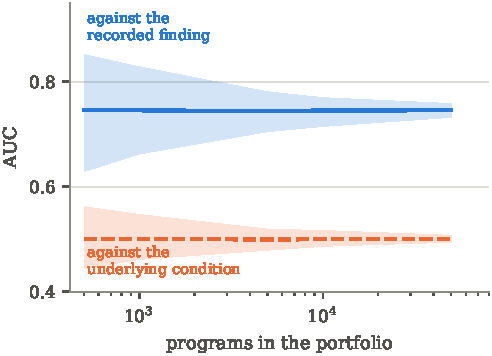
\includegraphics[width=0.6\textwidth]{exB3_finite.pdf}
\caption{\capFinite}
\label{fig:finite}
\end{figure}

\section{Empirical detail}\label{app:emp}

\subsection{Data acquisition and panel construction}

The Federal Audit Clearinghouse publishes the complete structured results of
every Single Audit submission as bulk files at
\url{https://www.fac.gov/data/download/}, without registration,
authentication or fee. Seven files were retrieved in September 2026 and cover
fiscal years 2016 onward. No free-text finding narratives, no restricted data
and no nonpublic records of any kind were used. The regulatory provisions
quoted are from Title~2 of the Code of Federal Regulations; the 2023 annual
edition is the one in force over the sample period.

The unit of analysis is the auditee--program--year. A ``program'' is the
regulatory program unit: a cluster of programs where one exists, otherwise a
single assistance listing number. That follows 2~CFR 200.518(b)(3), under
which ``a cluster of programs is treated as one program'' for the Type~A
determination, so the unit matches the one the rules operate on. The window
is fiscal years 2016 through 2023, restricted to audits whose fiscal year began
within the period governed by the \$750,000 audit and Type~A thresholds in
200.501(a) and 200.518(b)(1) as they stood before the 2024 revision, which
raised both to \$1,000,000 for fiscal years beginning on or after 1~October
2024 \citep{omb2024}. The panel ends before that revision takes effect, so a
single threshold regime governs throughout.

Table~\ref{tab:sample} shows how the panel narrows and why a missing prior
year is not coded as a clean one. The panel distinguishes a resolved
prior-year observation with no finding from the absence of any prior-year
record for that program: of the \nPanelRows{} program-years, \nSone{} have a
resolved prior-year finding and \nStwo{} a resolved prior-year clean result;
the remainder are excluded rather than recoded. Sample~A restricts further to
program-years in which the program was audited as major in both years. It
holds the major-program-selection channel fixed. It does not hold audit
intensity or condition-specific observation fixed, and cannot, for the reason
given in Section~\ref{sec:regime}: the follow-up requirement applies within
Sample~A.

Two definitions of ``repeat'' are used. The primary one is the auditor's own
coding. The secondary one is a validated historical link: a finding whose
cited prior reference number appears as a finding reference recorded for the
same auditee and program in the immediately preceding year. Of the
\nLinkFlagged{} findings that cite a prior-finding reference, \nLinkResolved{}
resolve this way, \nLinkPct{}~percent. Non-resolution has innocent causes: the
prior finding may sit two or more years back, may be recorded against a
different program unit, or may carry a renumbered reference. Neither measure
is a gold standard, so both are reported. Intervals throughout are 95 percent
cluster bootstrap with \nBootReps{} replications, resampling \nNAuditees{}
auditees together with their full histories, seed \nBootSeed{}.

\subsection{Every specification}

Table~\ref{tab:specs} collects the risk differences under all five
specifications reported anywhere in this paper. The first row is the primary
result of Table~\ref{tab:fourstate}. The second substitutes the validated
historical link for the auditor's repeat flag. This definition mechanically
forces both repeat states to zero for program-years with no prior finding, so
its risk differences are interpretable and its risk ratios are not. It has a
second consequence, which the table makes explicit. Under the auditor's flag,
every recorded finding is either marked a repeat or is not, so the four
outcome states exhaust the possibilities and their risk differences add to the
difference in ``any finding''. Under the validated link they do not. A
program-year whose findings were all flagged as repeats, none of which
resolves to a same-program prior-year reference, has recorded no new finding
and no \emph{validated} repeat, and therefore falls outside all four states.
That fifth state occurs in \nVlinkFifthNoPrior{} of program-years with no
prior finding and \nVlinkFifthPrior{} of those with one, a difference of
\nVlinkFifth{}, which is exactly the gap between the four state columns and
``any finding'' in that row. It is given its own column rather than absorbed
anywhere, and the sum is checked in every row.

The third row drops the requirement that the program be audited as major in
both years, using all program-years with a resolved prior observation. The
fourth restricts to transitions whose Clearinghouse provenance is stable across
the two years, which addresses the possibility that repeat-flag capture differs
between the two administering systems that operated during the window; that
restriction excludes \nProvExcluded{} transitions. The fifth uses the
three-year cumulative history rule, requiring resolved observations at $t-1$,
$t-2$ and $t-3$. Across all five, the any-new margin is the most stable
quantity in the table.

\subsection{The allocation of mixed periods}

Table~\ref{tab:zeta} gives the full sensitivity of the ``percent due to
recurrence'' statistic to the treatment of program-periods that recorded both a
repeat and a new finding. $\zeta$ is the fraction of mixed periods counted as
recurrence. The $\zeta = 1$ row gives \nNineZeroNine{}~percent; the $\zeta = 0$
row gives \nZetaLo{}~percent. The arithmetic is not in doubt: the numerator
$\nDRonly{} + \zeta \cdot \nDBoth{}$ and the denominator \nDAny{} are read
directly off Table~\ref{tab:fourstate}. A correctly computed statistic can
still be uninformative, because the quantity it reports is fixed by the
allocation rule rather than by anything observed.

\subsection{Compliance-requirement categories}

The Clearinghouse records a requirement category for every reported
deficiency. It does not record which requirements applied to, or were tested
in, a given program-period; that universe is defined by the Compliance
Supplement, which is external to these data. A first-in-area hazard therefore
has no constructible denominator here, and none was constructed.

What can be said is descriptive and applies only to programs that recorded
findings in both years. Among those \nOverlapN{} Sample~A program-years,
\nOverlapShares{}~percent share at least one requirement category across the
two years; the mean Jaccard overlap between the two category sets is
\nOverlapJaccard{}; on average \nOverlapEntering{} categories enter and
\nOverlapExiting{} exit between the two years. These are descriptions of a
conditioned subset, not comparisons across history groups, and they carry no
implication about the rate at which problems appear in new requirement areas.

\subsection{Horizons beyond one year}

Results at $t+2$ and $t+3$ are not reported in the main text, and the reason
is structural rather than statistical. Following a program past $t+1$ requires
it to be audited as a major program again, and that is exactly the quantity
the regulation makes depend on the finding record: a prior finding can block
low-risk Type~A status and so make recoverage more likely. The programs that
can be followed are therefore not a random subset of the programs one would
want to follow, and the selection runs in the direction that would flatter a
persistence interpretation.

The attrition is severe. Of \nHorizonNone{} Sample~A finding-years with
resolved follow-up at $t+1$, \nHorizonNtwo{} can be followed to $t+2$ and
\nHorizonNthree{} to $t+3$, losses of \nHorizonLossTwo{} and
\nHorizonLossThree{}~percent. Across those shrinking and increasingly selected
samples the explicit-repeat rate falls from \nHorizonRepeatOne{} at $t+1$ to
\nHorizonRepeatThree{} at $t+3$. That decline is what both a decay story and a
selection story predict, and the design cannot separate them, which is why the
numbers are recorded here rather than interpreted.

\subsection{Data and code availability}

Reproduction requires the seven bulk files, a build of the
auditee--program--year panel following the definitions above, and estimation
of the outcome shares with cluster-bootstrap intervals as described. The panel
construction, the four-state decomposition, the cluster bootstrap and the
simulations reported in Sections~\ref{sec:design} and \ref{sec:scoring} are
implemented in Python and DuckDB with a fixed master seed. The quantities
reported from simulation are either exact calculations or Monte Carlo results
from a single prespecified configuration; no parameter search was performed,
and each table states which of the two it is. The full analysis code, the
intermediate panel and cryptographic digests of every input and output will be
deposited with the journal on conditional acceptance and retained for at least
seven years.

\begin{table}[tbp]
\centering
\caption{\textbf{How the sample was built, and what was left out.} The upper
panel narrows the panel to program-years in which the same program can be
observed in two consecutive years with its major-program status known in both.
The lower panel is the reason the paper does not simply code a missing prior
year as a clean year. In 366,506 program-years --- 15.35 percent of the panel --- the
auditee filed an audit last year but this program does not appear in it. Those
program-years record a finding 3.26 percent of the time, which is not the rate of
a clean program. They are excluded rather than recoded, because the absence of a
record is not a clean result.}
\label{tab:sample}
\footnotesize
\setlength{\tabcolsep}{3pt}
\begin{tabular}{lrr}
\toprule
Step & Program-years & Excluded here \\
\midrule
All program-years in the panel & 2,387,511 &  \\
Within the \$750,000 regime (FY2016--2023) & 2,387,511 & 0 \\
With a resolved prior-year observation & 1,600,898 & 786,613 \\
Sample A: audited as a major program in both years & 206,926 & 1,393,972 \\
\bottomrule
\end{tabular}

\vspace{1.1em}

\footnotesize
\begin{tabular}{lrrrl}
\toprule
What the prior year looks like & Program-years & Share & \shortstack{Finding rate\\this year} & Treatment \\
\midrule
Prior year resolved, finding recorded & 66,131 & 2.77\% & 0.4723 & kept \\
Prior year resolved, no finding recorded & 1,534,767 & 64.28\% & 0.0206 & kept \\
Auditee filed last year; this program is not in that filing & 366,506 & 15.35\% & 0.0326 & excluded \\
No filing at all for this auditee last year & 160,861 & 6.74\% & 0.0706 & excluded \\
First year of the window (2016) & 259,246 & 10.86\% & 0.0462 & excluded \\
\bottomrule
\end{tabular}
\end{table}

\begin{table}[htbp]
\centering
\caption{Risk differences under every specification reported.}
\label{tab:specs}
\scriptsize
\setlength{\tabcolsep}{3pt}
\begin{tabular}{lrcccccc}
\toprule
& & \multicolumn{4}{c}{Mutually exclusive outcome states} & & \\
\cmidrule(lr){3-6}
Specification & $n$ & repeat only & new only & both & \shortstack{flagged repeat,\\ not linked} & any finding & any new finding \\
\midrule
Sample A, auditor flag (primary) & 206,926 & $+0.3073$ & $+0.0456$ & $+0.1488$ & --- & $+0.5017$ & $+0.1945$ \\
Sample A, validated link & 206,926 & $+0.2994$ & $+0.0491$ & $+0.1454$ & $+0.0079$ & $+0.5017$ & $+0.1945$ \\
All resolved transitions & 1,600,898 & $+0.2869$ & $+0.0617$ & $+0.1031$ & --- & $+0.4517$ & $+0.1648$ \\
Stable provenance & 167,017 & $+0.2935$ & $+0.0510$ & $+0.1439$ & --- & $+0.4885$ & $+0.1949$ \\
Three-year history & 94,360 & $+0.1959$ & $+0.0774$ & $+0.0942$ & --- & $+0.3674$ & $+0.1716$ \\
\bottomrule
\end{tabular}
\tablenotes{The primary row is
the one in Table~\ref{tab:fourstate}. The validated-link row mechanically forces
the repeat states to zero for program-years with no prior finding, so its risk
differences are usable and its ratios are not. It also opens a fifth outcome
state: a period whose findings were all auditor-flagged repeats, none of which
resolves to a same-program prior-year reference, records no new finding and no
validated repeat, and so falls outside all four. That column is empty for every
other specification, where the four states do exhaust the possibilities. In each
row the four state columns sum to ``any finding'', which the exhibit script
asserts on the unrounded values; the columns here are rounded independently, so
a row may add up one unit in the last place away from the total shown. The
any-new margin is the quantity that moves least across all five
specifications.}
\end{table}

\begin{table}[htbp]
\centering
\caption{The recurrence share as a function of a reporting convention. $\zeta$ is
the fraction of mixed program-periods --- those recording both a repeat and a
new finding --- counted as recurrence. Counting all of them gives
90.9~percent; counting none gives
61.2~percent. Nothing observable differs between the
two ends, which is why the paper reports the three-way split instead.}
\label{tab:zeta}
\small
\begin{tabular}{ccc}
\toprule
$\zeta$ & ``due to recurrence'' & ``first recorded'' \\
\midrule
0.00 & 61.2\% & 38.8\% \\
0.25 & 68.7\% & 31.3\% \\
0.50 & 76.1\% & 23.9\% \\
0.75 & 83.5\% & 16.5\% \\
1.00 & 90.9\% & 9.1\% \\
\bottomrule
\end{tabular}
\end{table}



\end{document}
